
The primer vector meta-algorithm was applied to some scenarios that represent generic maneuvers that may be of interest in LEO\@. These scenarios will be presented, together with an explanation of why they were chosen, and then solutions for each of them, under different orbital models, will be presented.

TODO present orbital models?

TODO redo tables with 0 eps, introduce eps, include N?

\section{Scenarios}

\subsection{Circle to Circle rendez-vous}

A maneuver scenario corresponding to a Hohmann transfer (under a two body model) was chosen. Firstly, because in the two body model, there is an analytical solution for the transfer, given in Section~\ref{sssec:hohmann}. And secondly, this is a simple scenario that highlights the difference between the different orbital models used in the work. The orbital parameters are given in Table~\ref{tab:hohmann_orb_elems}, as well as a 3D rendering of the scenario in Figure~\ref{fig:hohmann_scenario}. The transfer time was calculated analytically to correspond to the Hohmann transfer time.

\begin{table}[htbp]
    \centering
    \begin{tabular}{ccc} \toprule
        Element & Initial & Final \\ \midrule
        \(a\)      & \(7000.0\) km         & \(9000.0\) km   \\
        \(e\)      & \(0.0\)            & \(0.0\)        \\
        \(i\)      & \(51.0^\circ\)      & \(51.0^\circ\) \\
        \(\Omega\) & \(0.0^\circ\)   & \(0.0^\circ\)  \\
        \(\omega\) & \(0.0^\circ\)  & \(0.0^\circ\)  \\
        \(\theta\) & \(0.0^\circ\)  & \(180.0^\circ\)  \\ 
        Transfer time & \multicolumn{2}{c}{\(3560.541\)} \\\bottomrule
    \end{tabular}
    \caption{Orbital elements used for the Hohmann transfer case analysis}
    \label{tab:hohmann_orb_elems}
\end{table}

\begin{figure}[htbp]
    \centering
    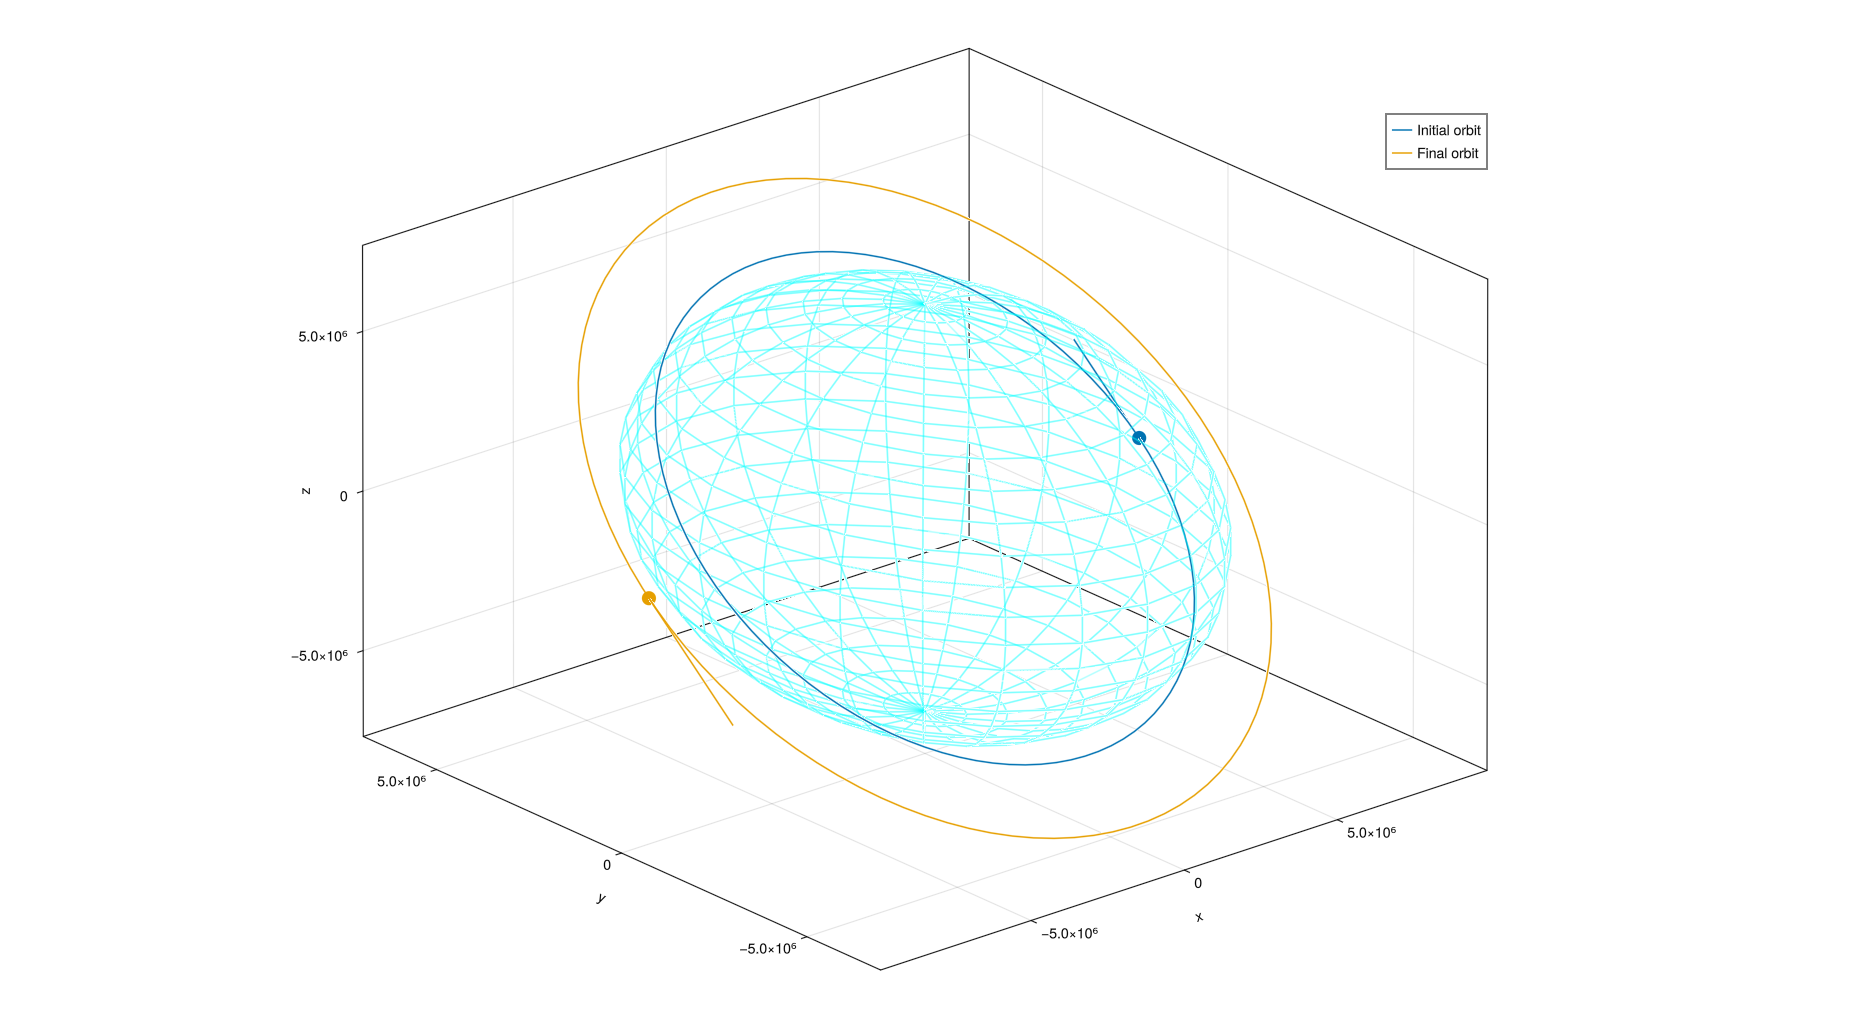
\includegraphics{../results/two_body/hohmann/scenario.png}
    \caption{Circle to Circle transfer scenario.}
    \label{fig:hohmann_scenario}
\end{figure}

\subsection{Noncoplanar rendez-vous}

A second, more challenging scenario is taken from \citeonline{interactive_primer_vector}, where a noncoplanar rendez-vous scenario is proposed and solved under the two body model. Again, the goal is validating the code against a published result under the two body model, and exploring how the optimal trajectory may be different under other more realistic models. The orbital parameters are given in Table~\ref{tab:noncop_rdv_orb_elems}, and multiple views of the scenario are shown in Figure~\ref{fig:noncop_rdv_scenario}. The transfer time is equal to two orbital periods of the target orbit.

\begin{table}[htbp]
    \centering
    \begin{tabular}{ccc} \toprule
        Element & Initial & Final \\ \midrule
        \(a\)      & \(6748.0\) km         & \(6778.0\) km   \\
        \(e\)      & \(0.0\)            & \(0.0\)        \\
        \(i\)      & \(5.0^\circ\)      & \(5.0^\circ\) \\
        \(\Omega\) & \(35.0^\circ\)   & \(35.0^\circ\)  \\
        \(\omega\) & \(0.0^\circ\)  & \(0.0^\circ\)  \\
        \(\theta\) & \(0.0^\circ\)  & \(293.71^\circ\)  \\ 
        Transfer time & \multicolumn{2}{c}{\(4500.0\)} \\\bottomrule
    \end{tabular}
    \caption{Orbital elements used for the Hohmann transfer case analysis}
    \label{tab:noncop_rdv_orb_elems}
\end{table}

\begin{figure}[htbp]
    \centering
    \begin{subfigure}{0.49\linewidth}
        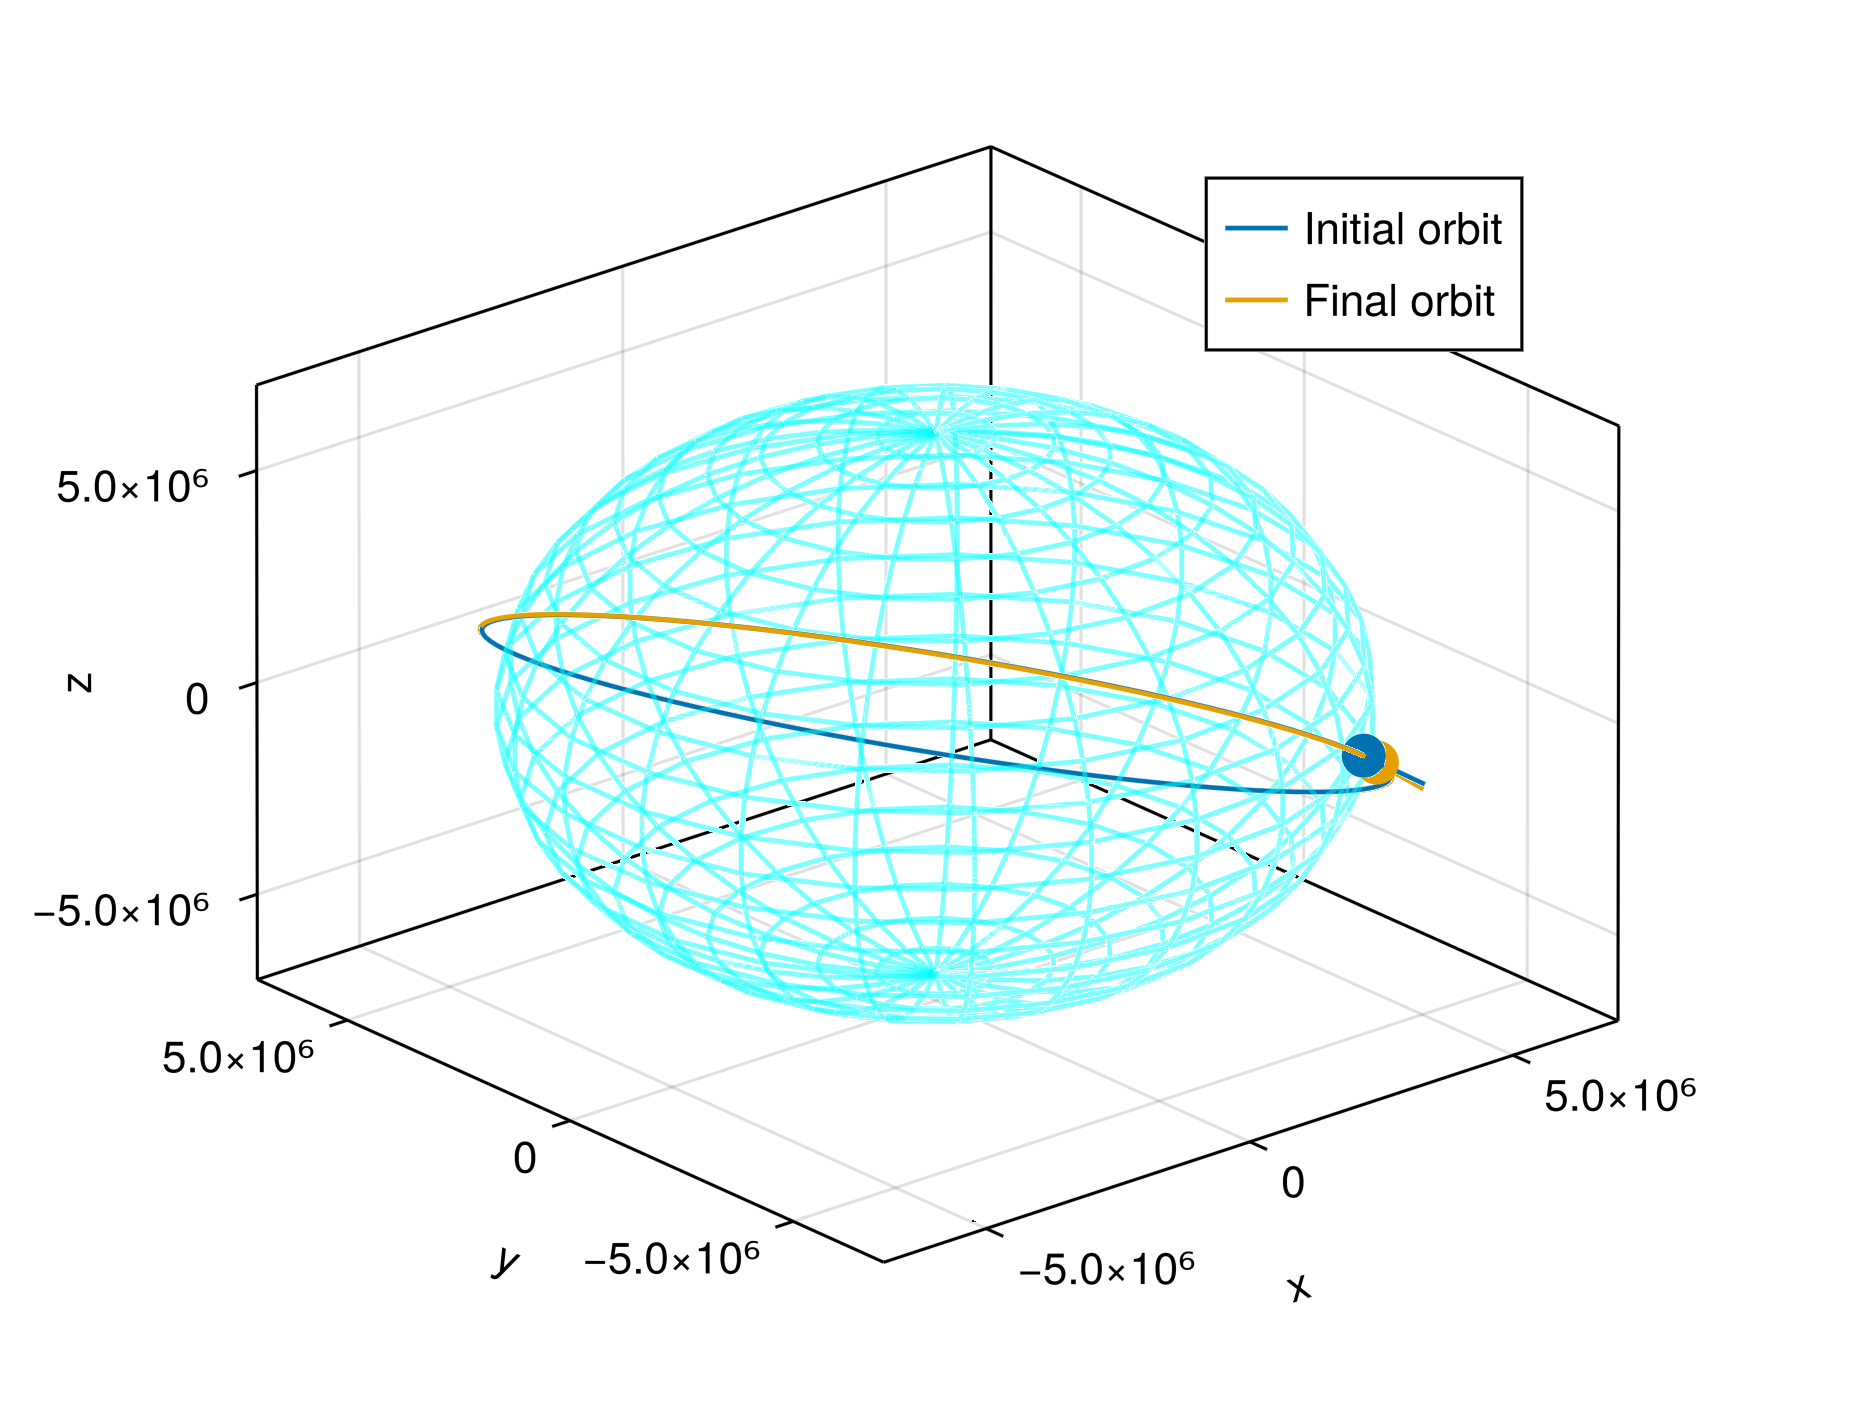
\includegraphics[width=\linewidth]{../results/two_body/ipv_noncop/scenario_3d.png}
        \caption{3D view.}
    \end{subfigure}
    \begin{subfigure}{0.49\linewidth}
        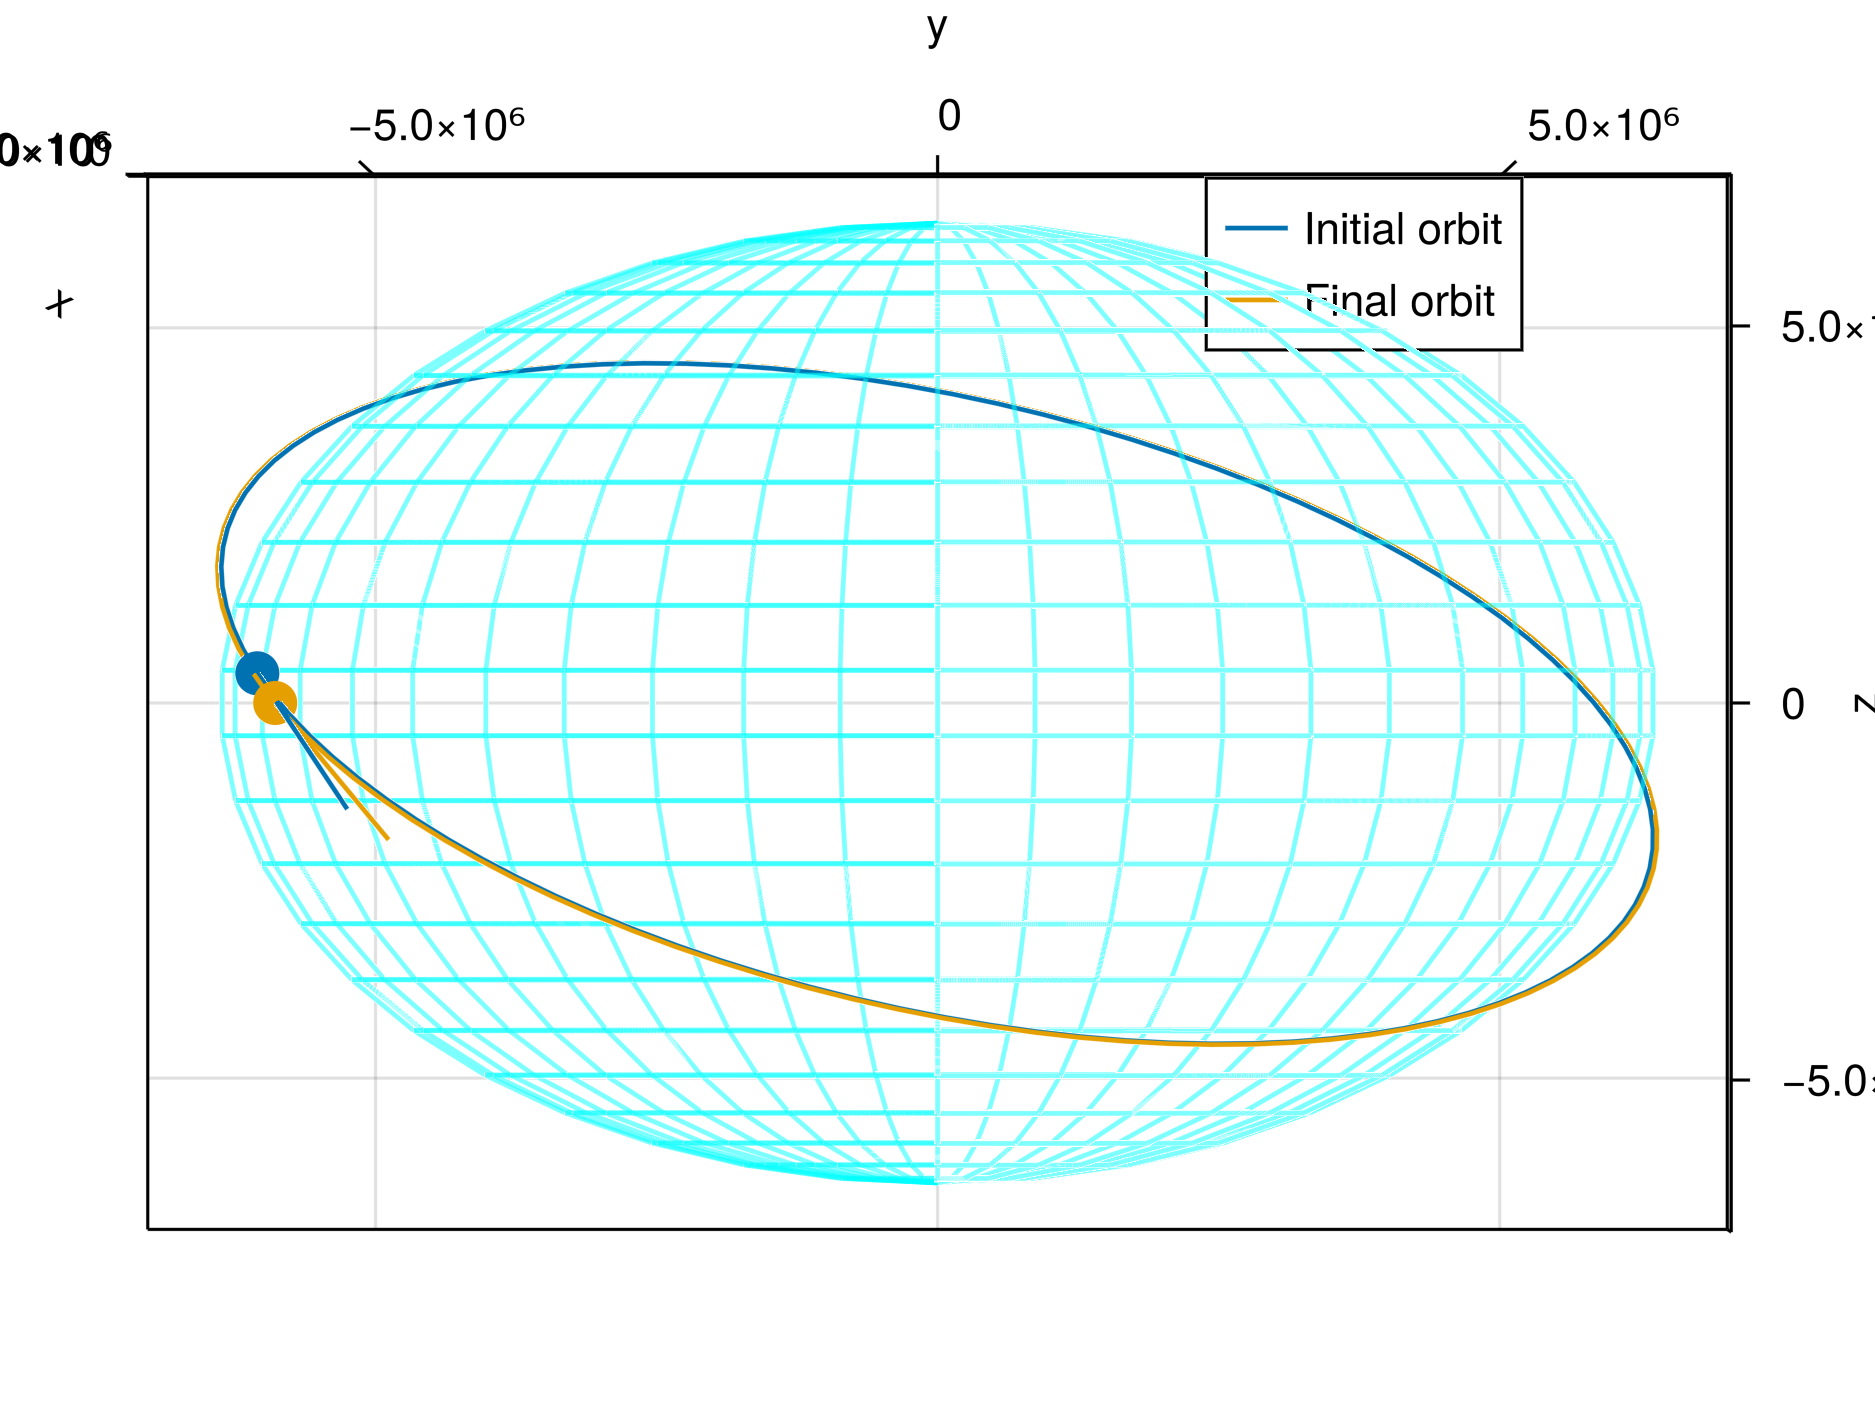
\includegraphics[width=\linewidth]{../results/two_body/ipv_noncop/scenario_x+.png}
        \caption{View from x+ axis.}
    \end{subfigure}
    \begin{subfigure}{0.49\linewidth}
        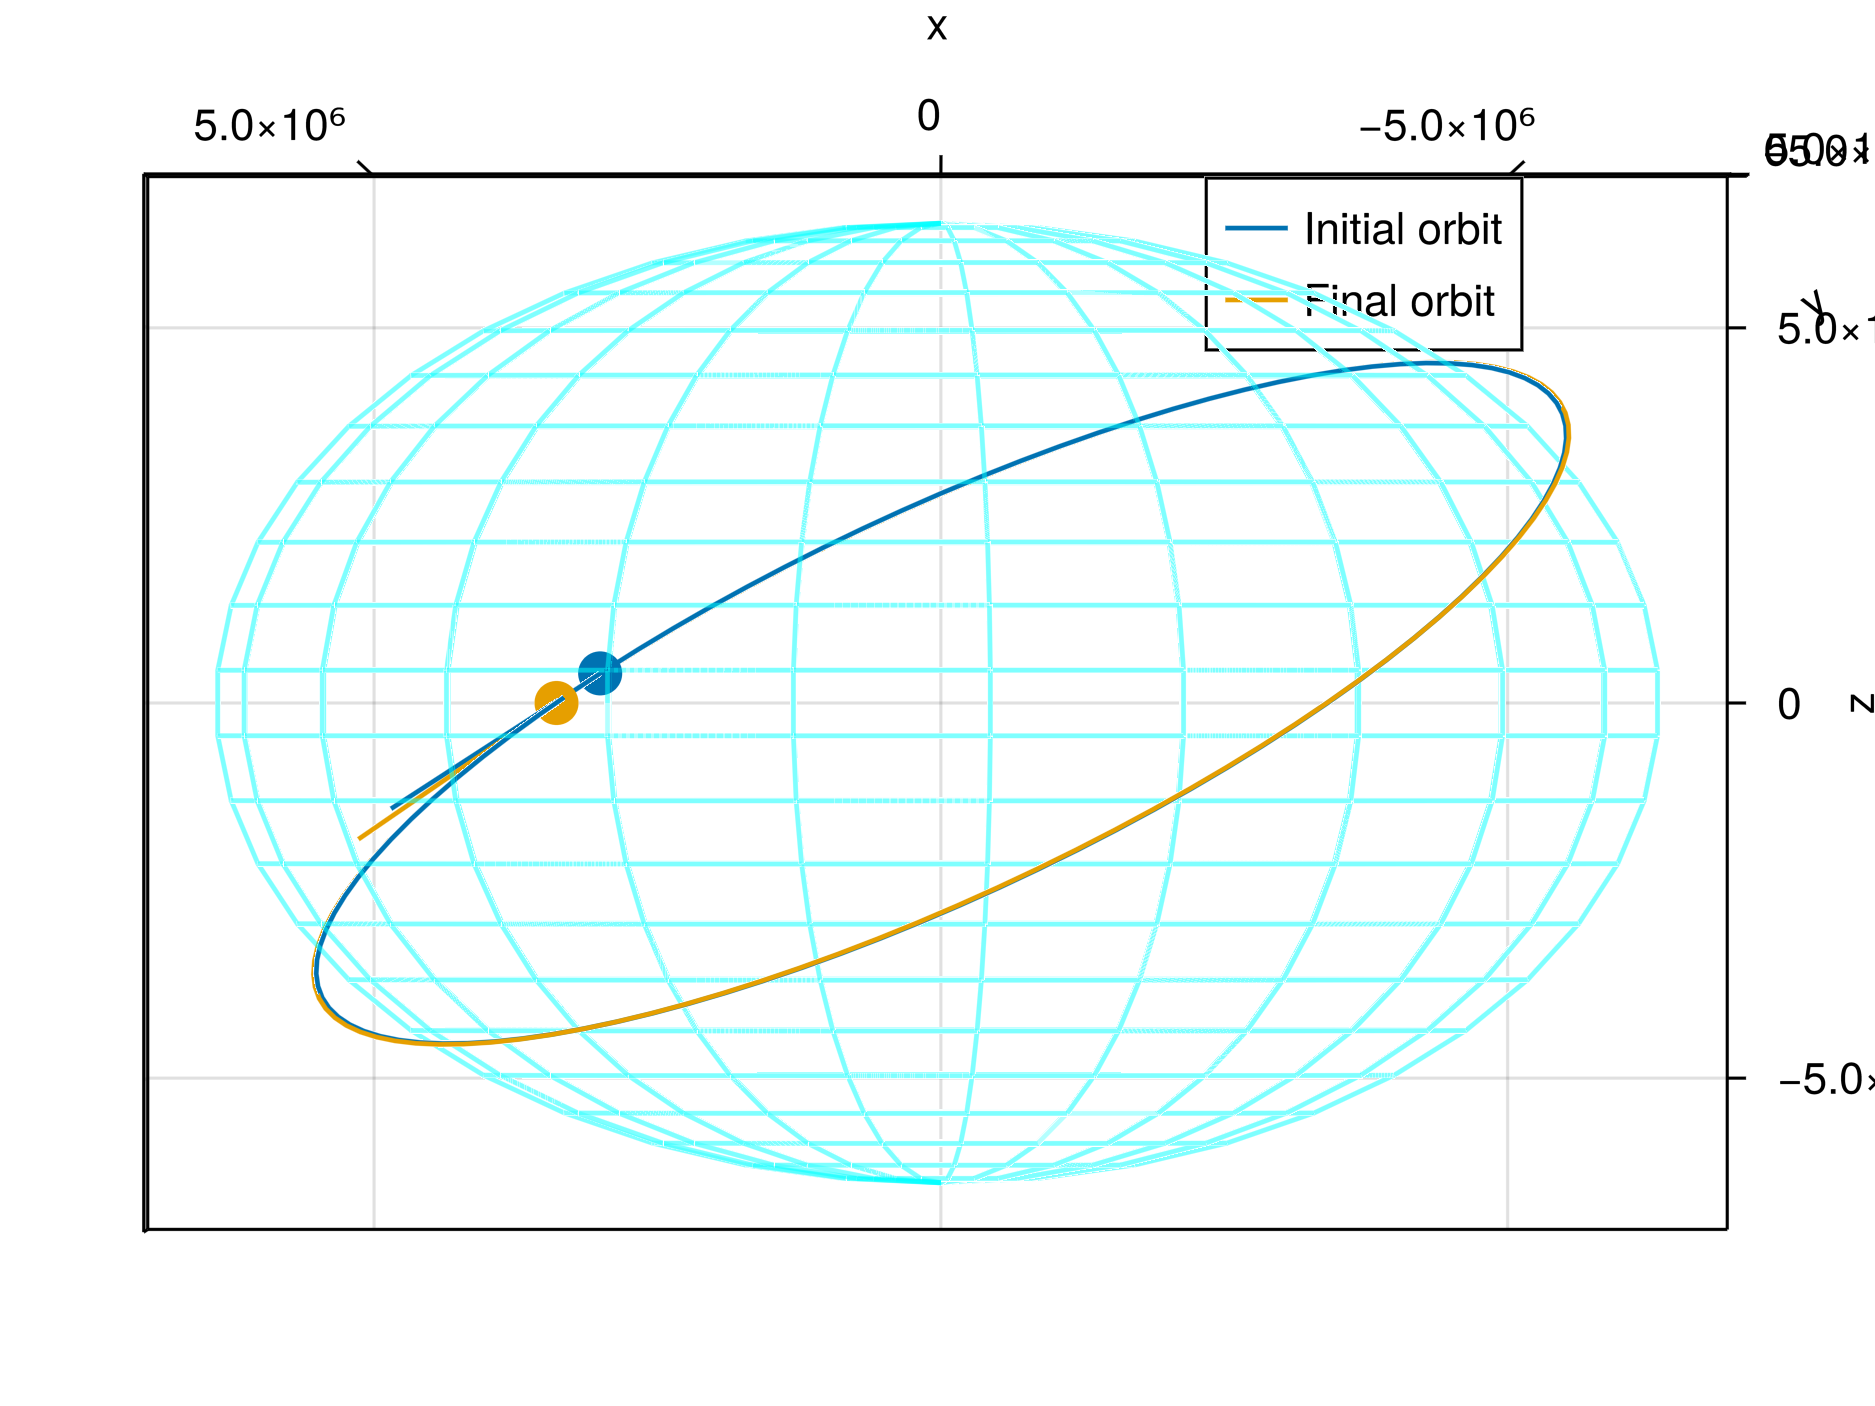
\includegraphics[width=\linewidth]{../results/two_body/ipv_noncop/scenario_y+.png}
        \caption{View from y+ axis.}
    \end{subfigure}
    \begin{subfigure}{0.49\linewidth}
        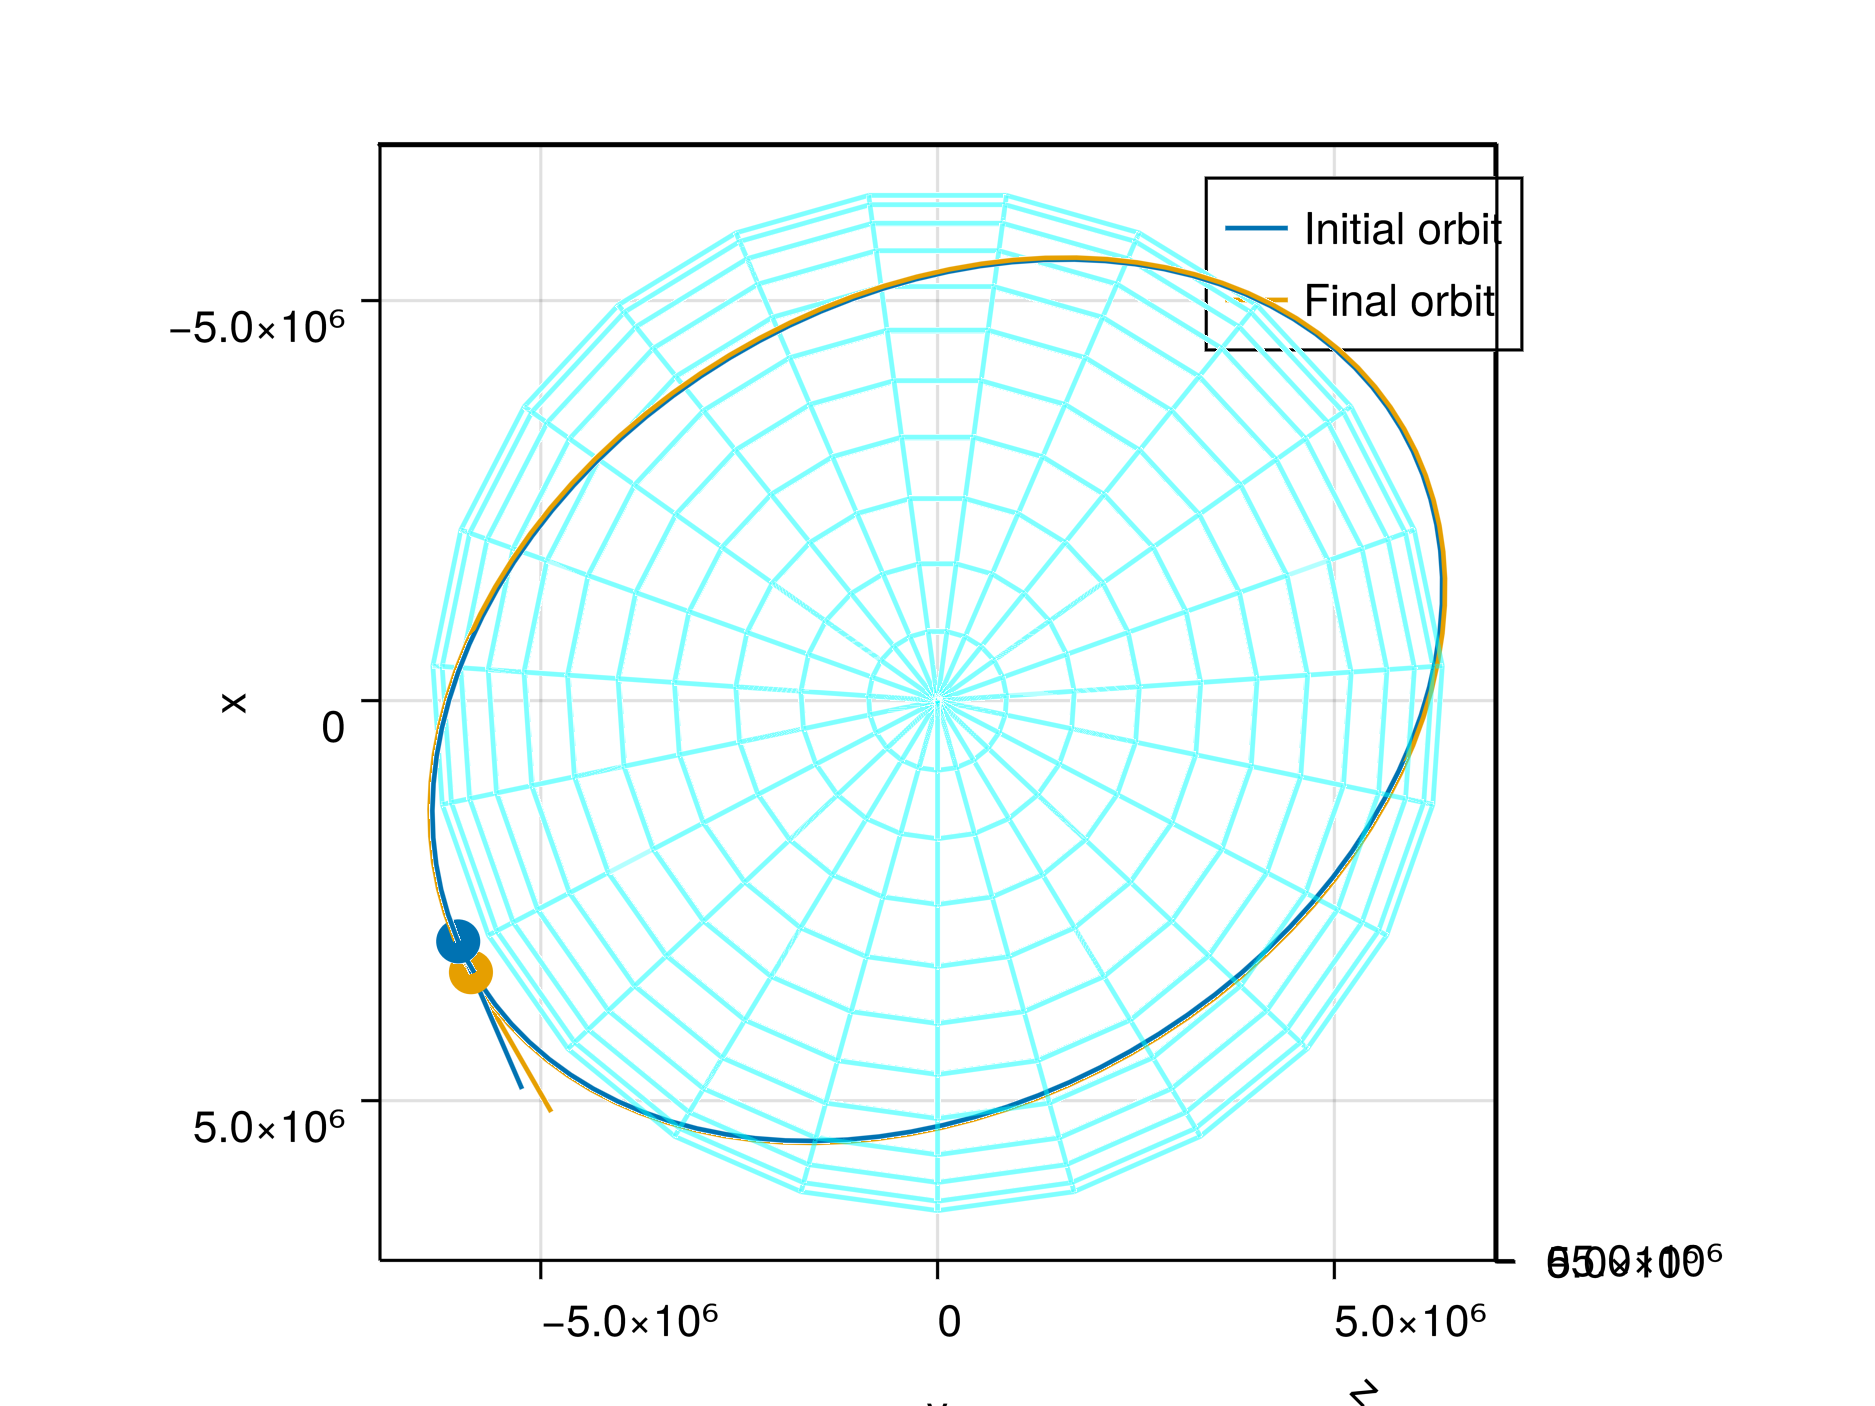
\includegraphics[width=\linewidth]{../results/two_body/ipv_noncop/scenario_z+.png}
        \caption{View from z+ axis.}
    \end{subfigure}
    \caption{Noncoplanar rendez-vous scenario 3D view and projections}
    \label{fig:noncop_rdv_scenario}
\end{figure}

\FloatBarrier
\section{Two Body}

The results for all scenarios under the two body model are presented in the following. All primer vector histories in this section were calculated with the Glandorf, STM and ODE methods, to numerically show they are equivalent. In all primer vector plots, vertical dashed lines indicate impulse times.

TODO Introdu ODE method

\subsection{Circle to Circle}

The circle to circle transfer scenario was first optimized for an \texttt{ICI} maneuver sequence. The results can be seen in Table~\ref{tab:tb_c2c_ICI_tab}, the primer vector trajectory can be seen in Figure~\ref{fig:tb_c2c_ICI_pv}, and the views of the optimized trajectory, in Figure~\ref{fig:tb_c2c_ICI_figs}. It can be seen that impulses at the starting and ending condition are capable of satisfying the necessary optimality conditions, and the analytical Hohmann of \(\Delta v_H = 887.56199 m/s\), computed from Equation~\eqref{eq:hohmann_deltav}, has been attained.

TODO try CICIC???

\begin{table}[htpb]
    \centering
    \begin{tabular}{cccc} \toprule
    \multicolumn{2}{c}{\textbf{Maneuver type}} & \multicolumn{2}{c}{ICI} \\ \midrule
    \(L\) (m) & \(T\) (s) & \(\varepsilon\) & \(\Delta x_{f}\) (m)    \\ \midrule
    8.0e6          & 1.0          & 0.0                & 0.0                        \\ \midrule
    \(\max \lVert p \rVert\) & 1.0     & \textbf{Diagnostic}   & Local optimum        \\ \midrule
    \textbf{Impulse} & \(t\) (s) & \(\Delta v\) (m/s) & \(1 - p \cdot \hat{u}\) \\ \midrule
    1                 & 0.0          & 457.74489             & 0.0                    \\
    2                 & 3560.54079          & 429.8171             & 0.0                    \\\midrule
    \textbf{Total}   & 3560.54079          & 887.56199             &                     \\ \bottomrule   
    \end{tabular}
    \caption{Summary of optimization for two body circle to circle \texttt{ICI} rendez-vous.}
    \label{tab:tb_c2c_ICI_tab}
\end{table}

\begin{figure}[htbp]
    \centering
    \begin{subfigure}{0.49\linewidth}
        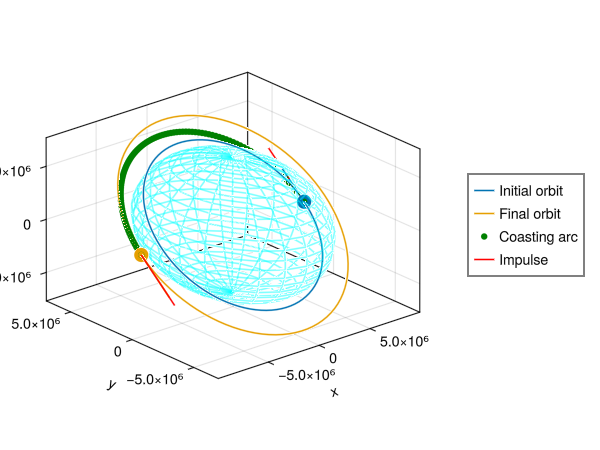
\includegraphics[width=\linewidth]{../results/two_body/hohmann/ICI_3d.png}
        \caption{3D view.}
    \end{subfigure}
    \begin{subfigure}{0.49\linewidth}
        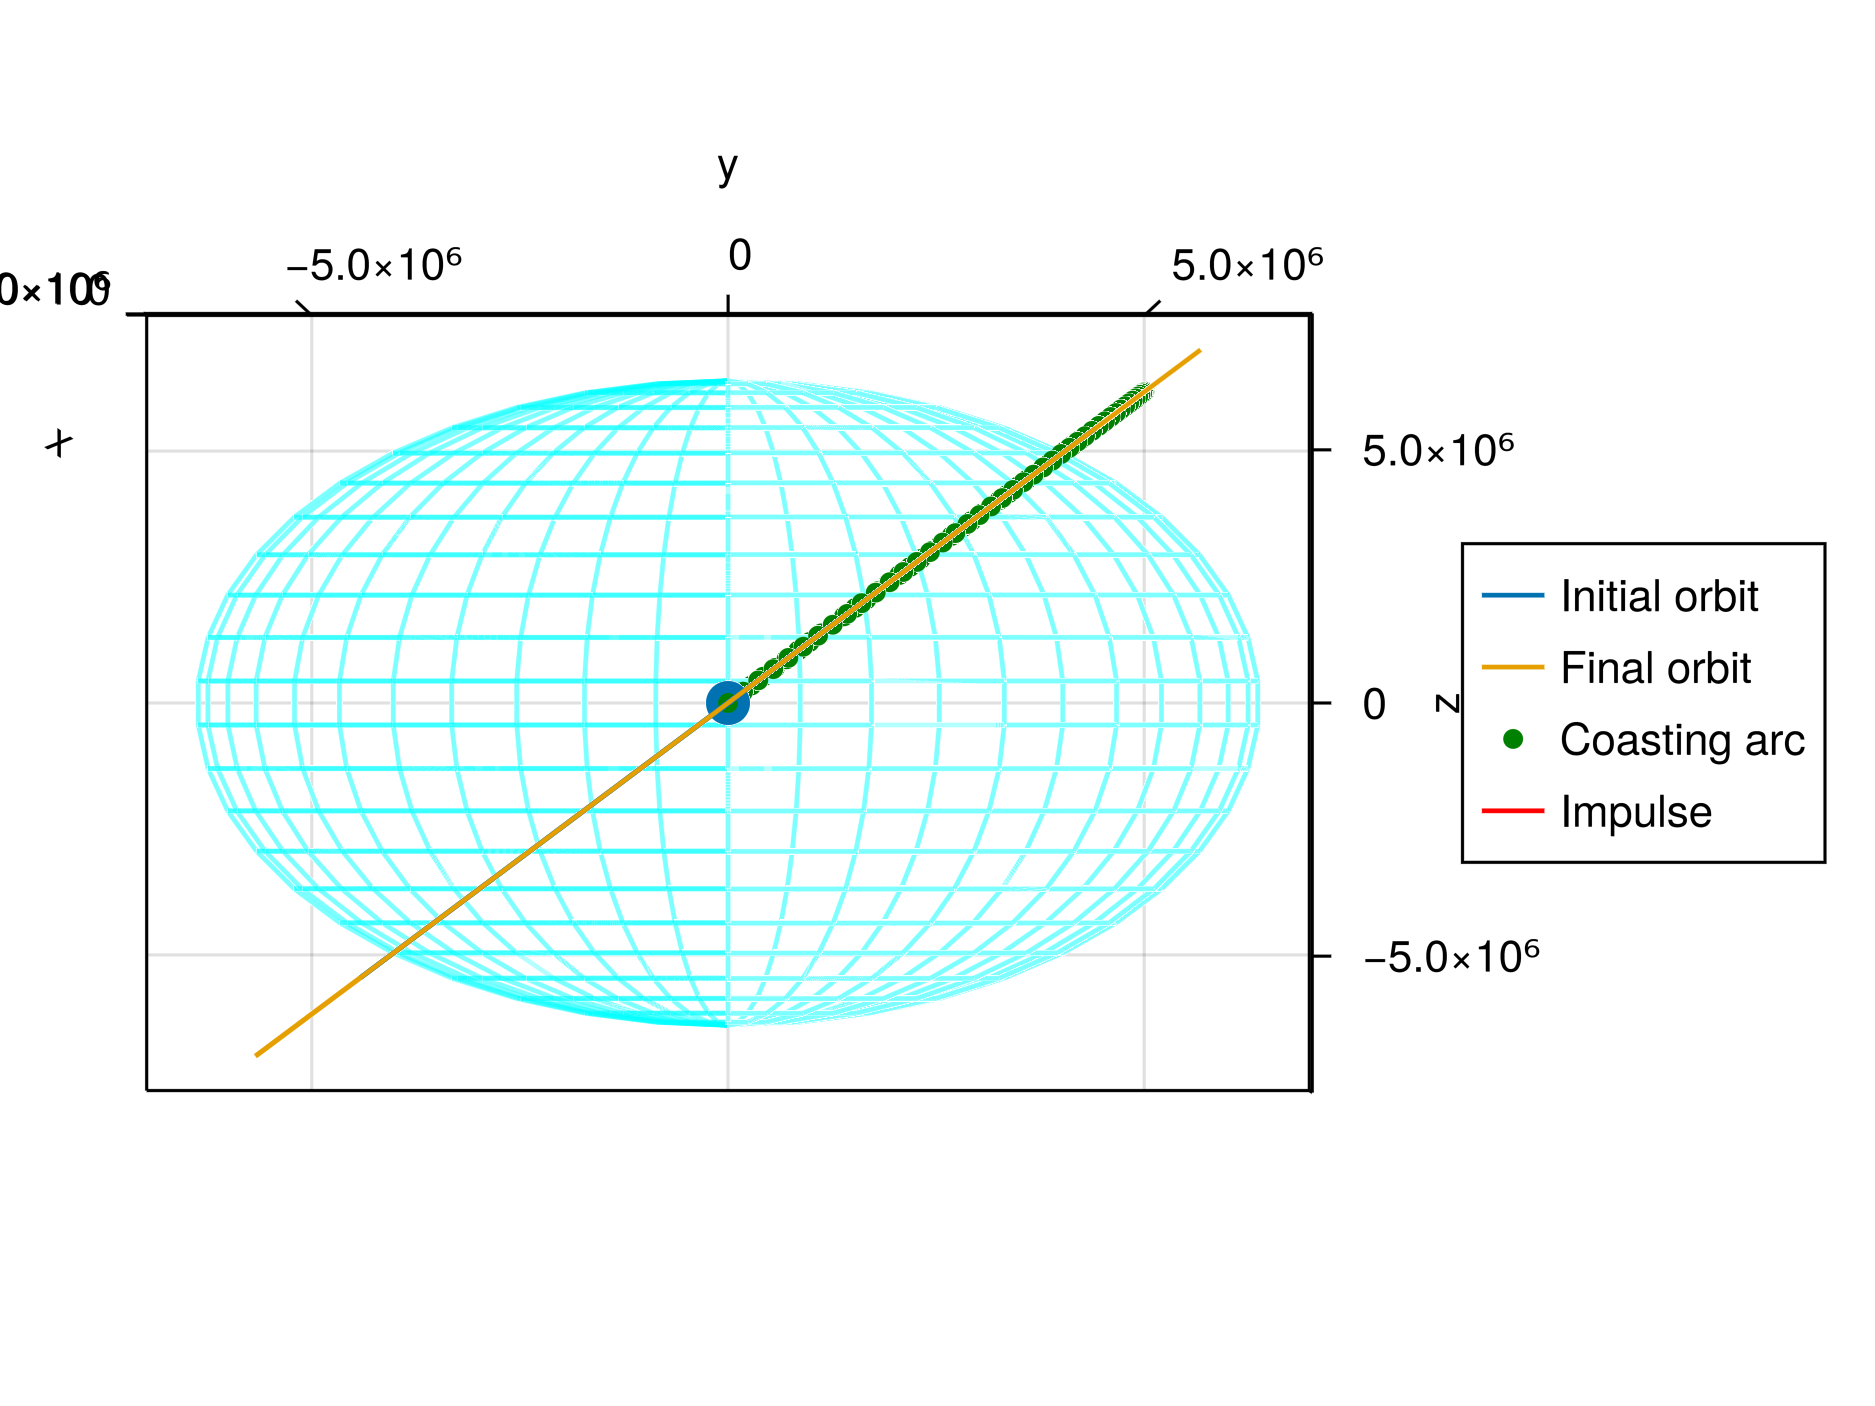
\includegraphics[width=\linewidth]{../results/two_body/hohmann/ICI_x+.png}
        \caption{View from x+ axis.}
    \end{subfigure}
    \begin{subfigure}{0.49\linewidth}
        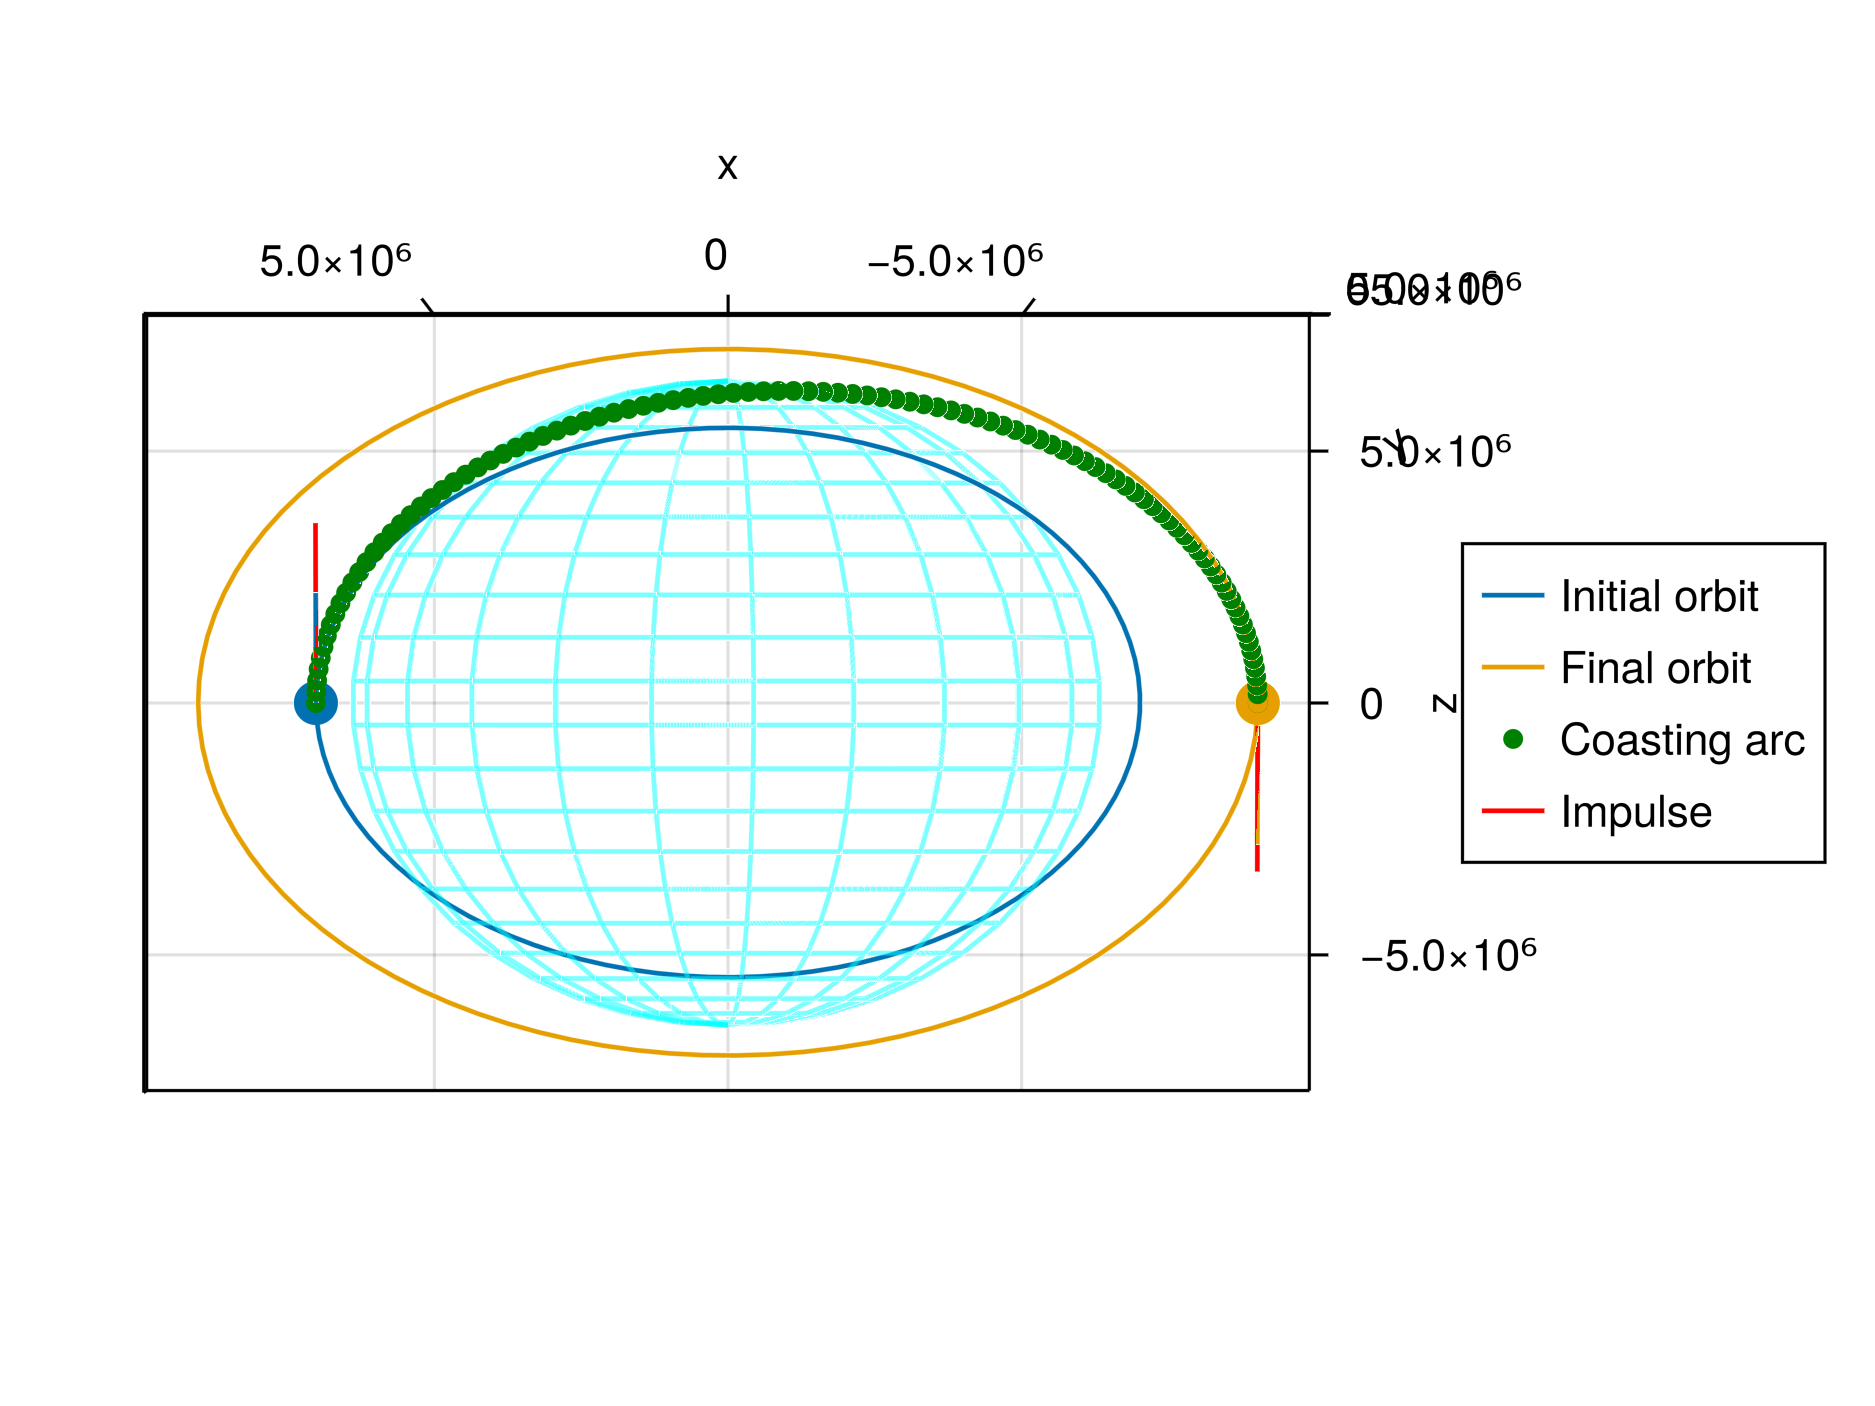
\includegraphics[width=\linewidth]{../results/two_body/hohmann/ICI_y+.png}
        \caption{View from y+ axis.}
    \end{subfigure}
    \begin{subfigure}{0.49\linewidth}
        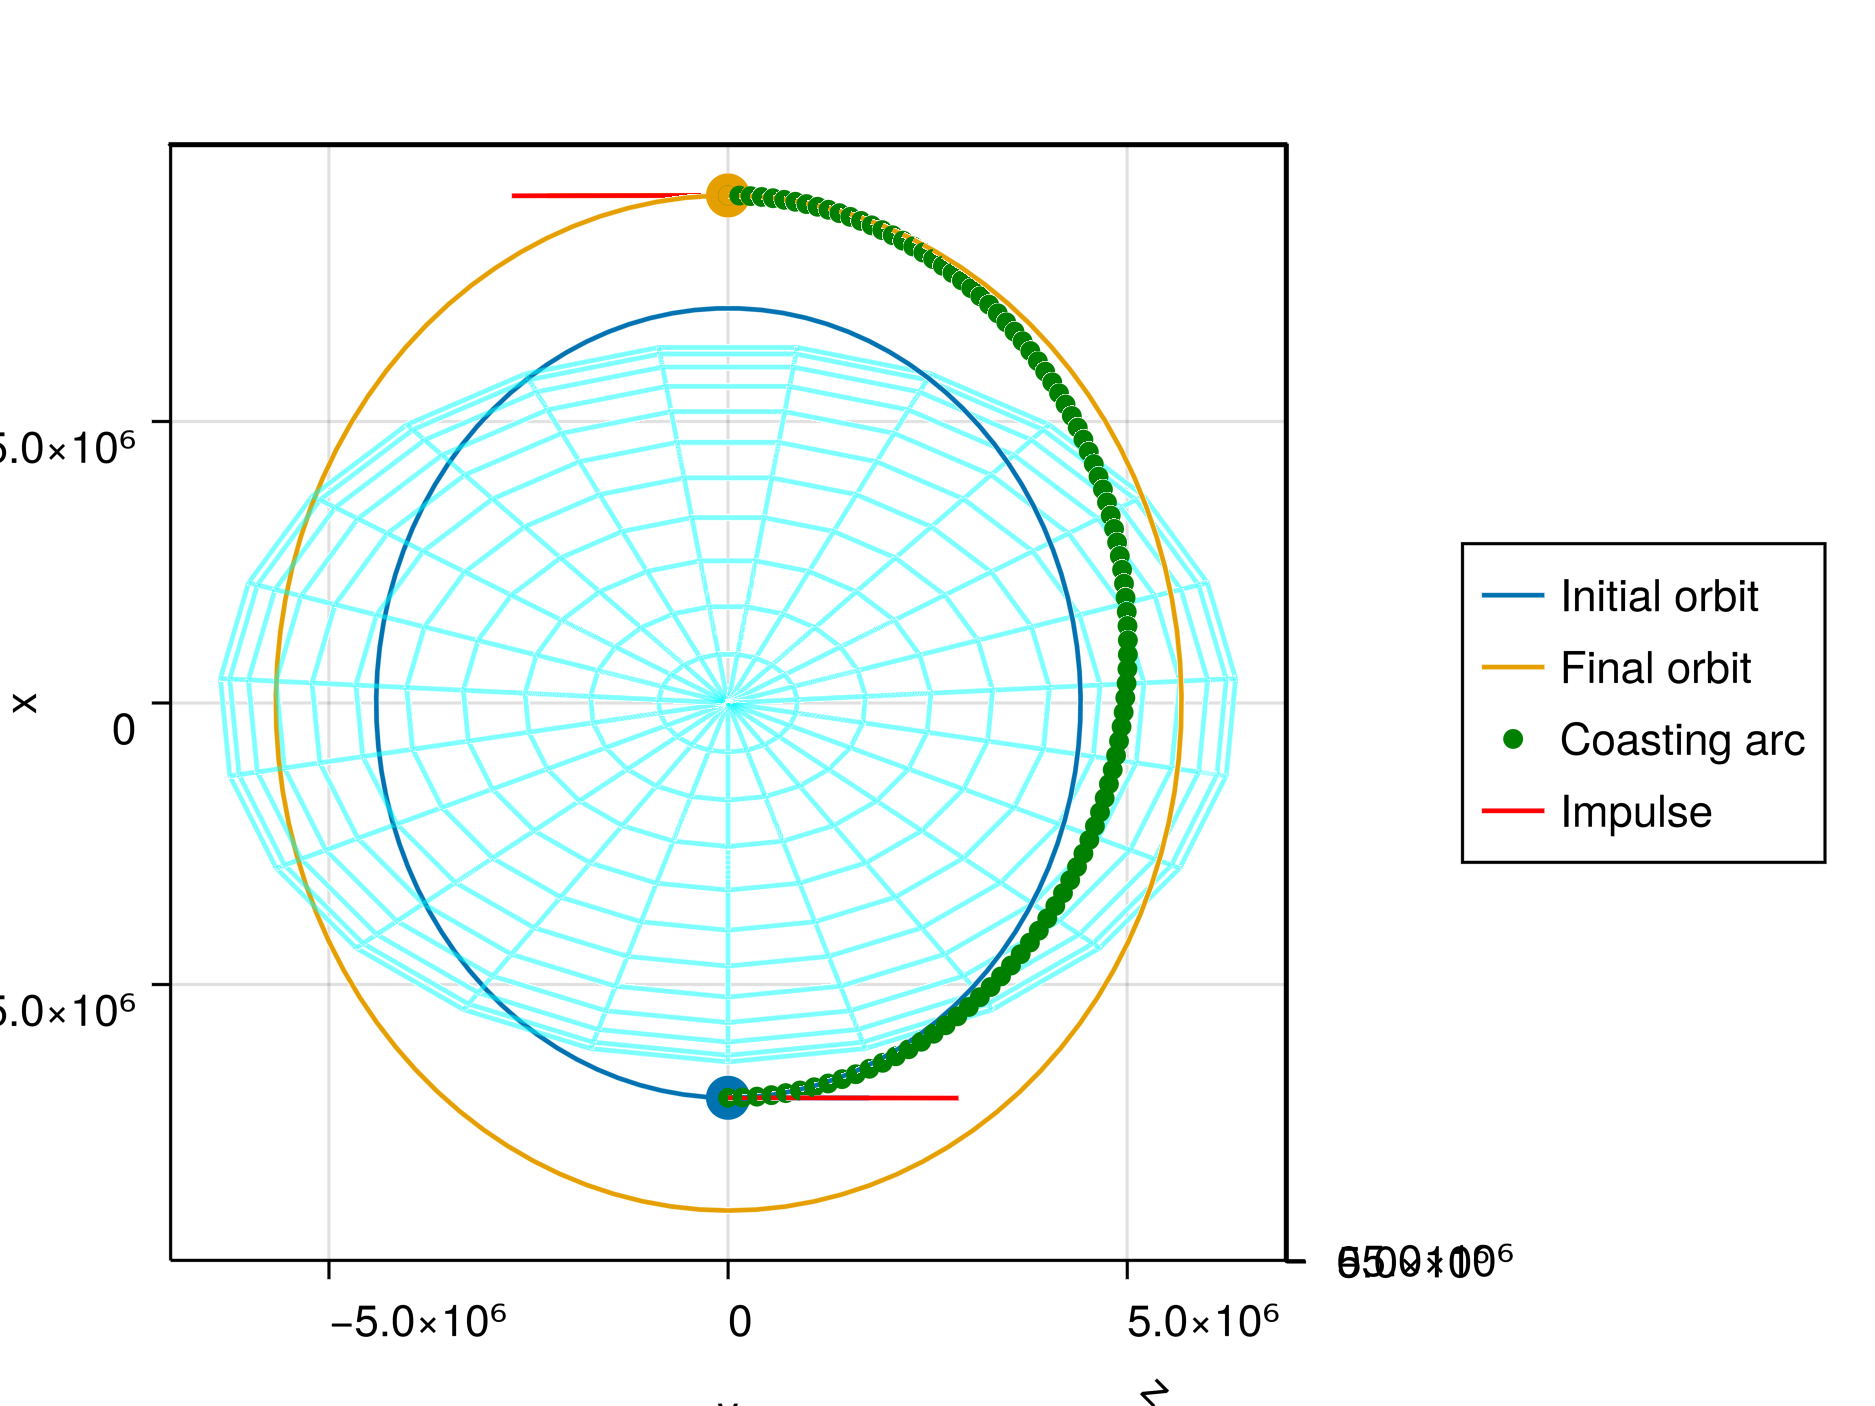
\includegraphics[width=\linewidth]{../results/two_body/hohmann/ICI_z+.png}
        \caption{View from z+ axis.}
    \end{subfigure}
    \caption{Circle to circle \texttt{ICI} maneuver 3D view and projections}
    \label{fig:tb_c2c_ICI_figs}
\end{figure}

\begin{figure}[htbp]
    \centering
    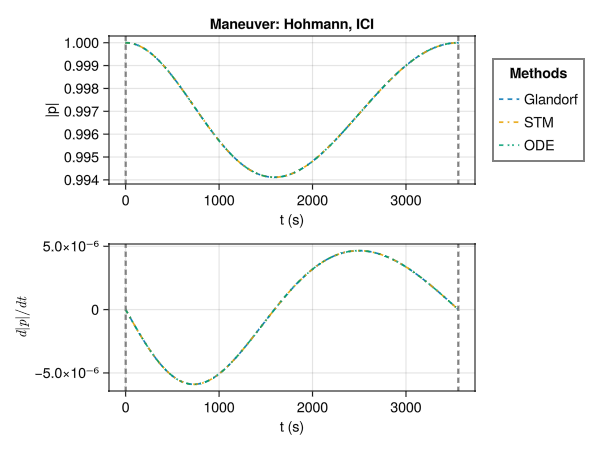
\includegraphics[width=\linewidth]{../results/two_body/hohmann/ICI_primer_vector.png}
    \caption{Primer vector trajectory for two body circle to circle \texttt{ICI} rendez-vous.}
    \label{fig:tb_c2c_ICI_pv}
\end{figure}

\subsection{Noncoplanar rendez-vous}

The more complex noncoplanar rendez-vous case was optimized with an \texttt{ICI} maneuver at first. The maneuver's summary, primer vector trajectory, and spatial views can be seen in Table~\ref{tab:tb_ncop_ICI_tab}, Figure~\ref{fig:tb_ncop_ICI_pv} and Figure~\ref{fig:tb_ncop_ICI_figs}. The primer vector history shows that this is a local optimum, but physical intuition suggests that there are less aggressive maneuvers that can solve the maneuver problem. In order to find better optima, the problem must be relaxed: the introduction of initial and final coasts increases the degrees of freedom of the control, possibly allowing for a better cost.

\begin{table}[htpb]
    \centering
    \begin{tabular}{cccc} \toprule
    \multicolumn{2}{c}{\textbf{Maneuver type}} & \multicolumn{2}{c}{ICI} \\ \midrule
    \(L\) (m) & \(T\) (s) & \(\varepsilon\) & \(\Delta x_{f}\) (m)    \\ \midrule
    6.7631e6          & 11107.158          & 1.00e-06                & 0.0                        \\ \midrule
    \(\max \lVert p \rVert\) & 1.0     & \textbf{Diagnostic}   & Local optimum        \\ \midrule
    \textbf{Impulse} & \(t\) (s) & \(\Delta v\) (m/s) & \(1 - p \cdot \hat{u}\) \\ \midrule
    1                 & 0.0          & 11740.94035             & -0.0                    \\
    2                 & 11107.1576          & 11708.69678             & -0.0                    \\\midrule
    \textbf{Total}   & 11107.1576          & 23449.63713             &                     \\ \bottomrule   
    \end{tabular}
    \caption{Summary of optimization for two body noncoplanar \texttt{ICI} rendez-vous.}
    \label{tab:tb_ncop_ICI_tab}
\end{table}

\begin{figure}[htbp]
    \centering
    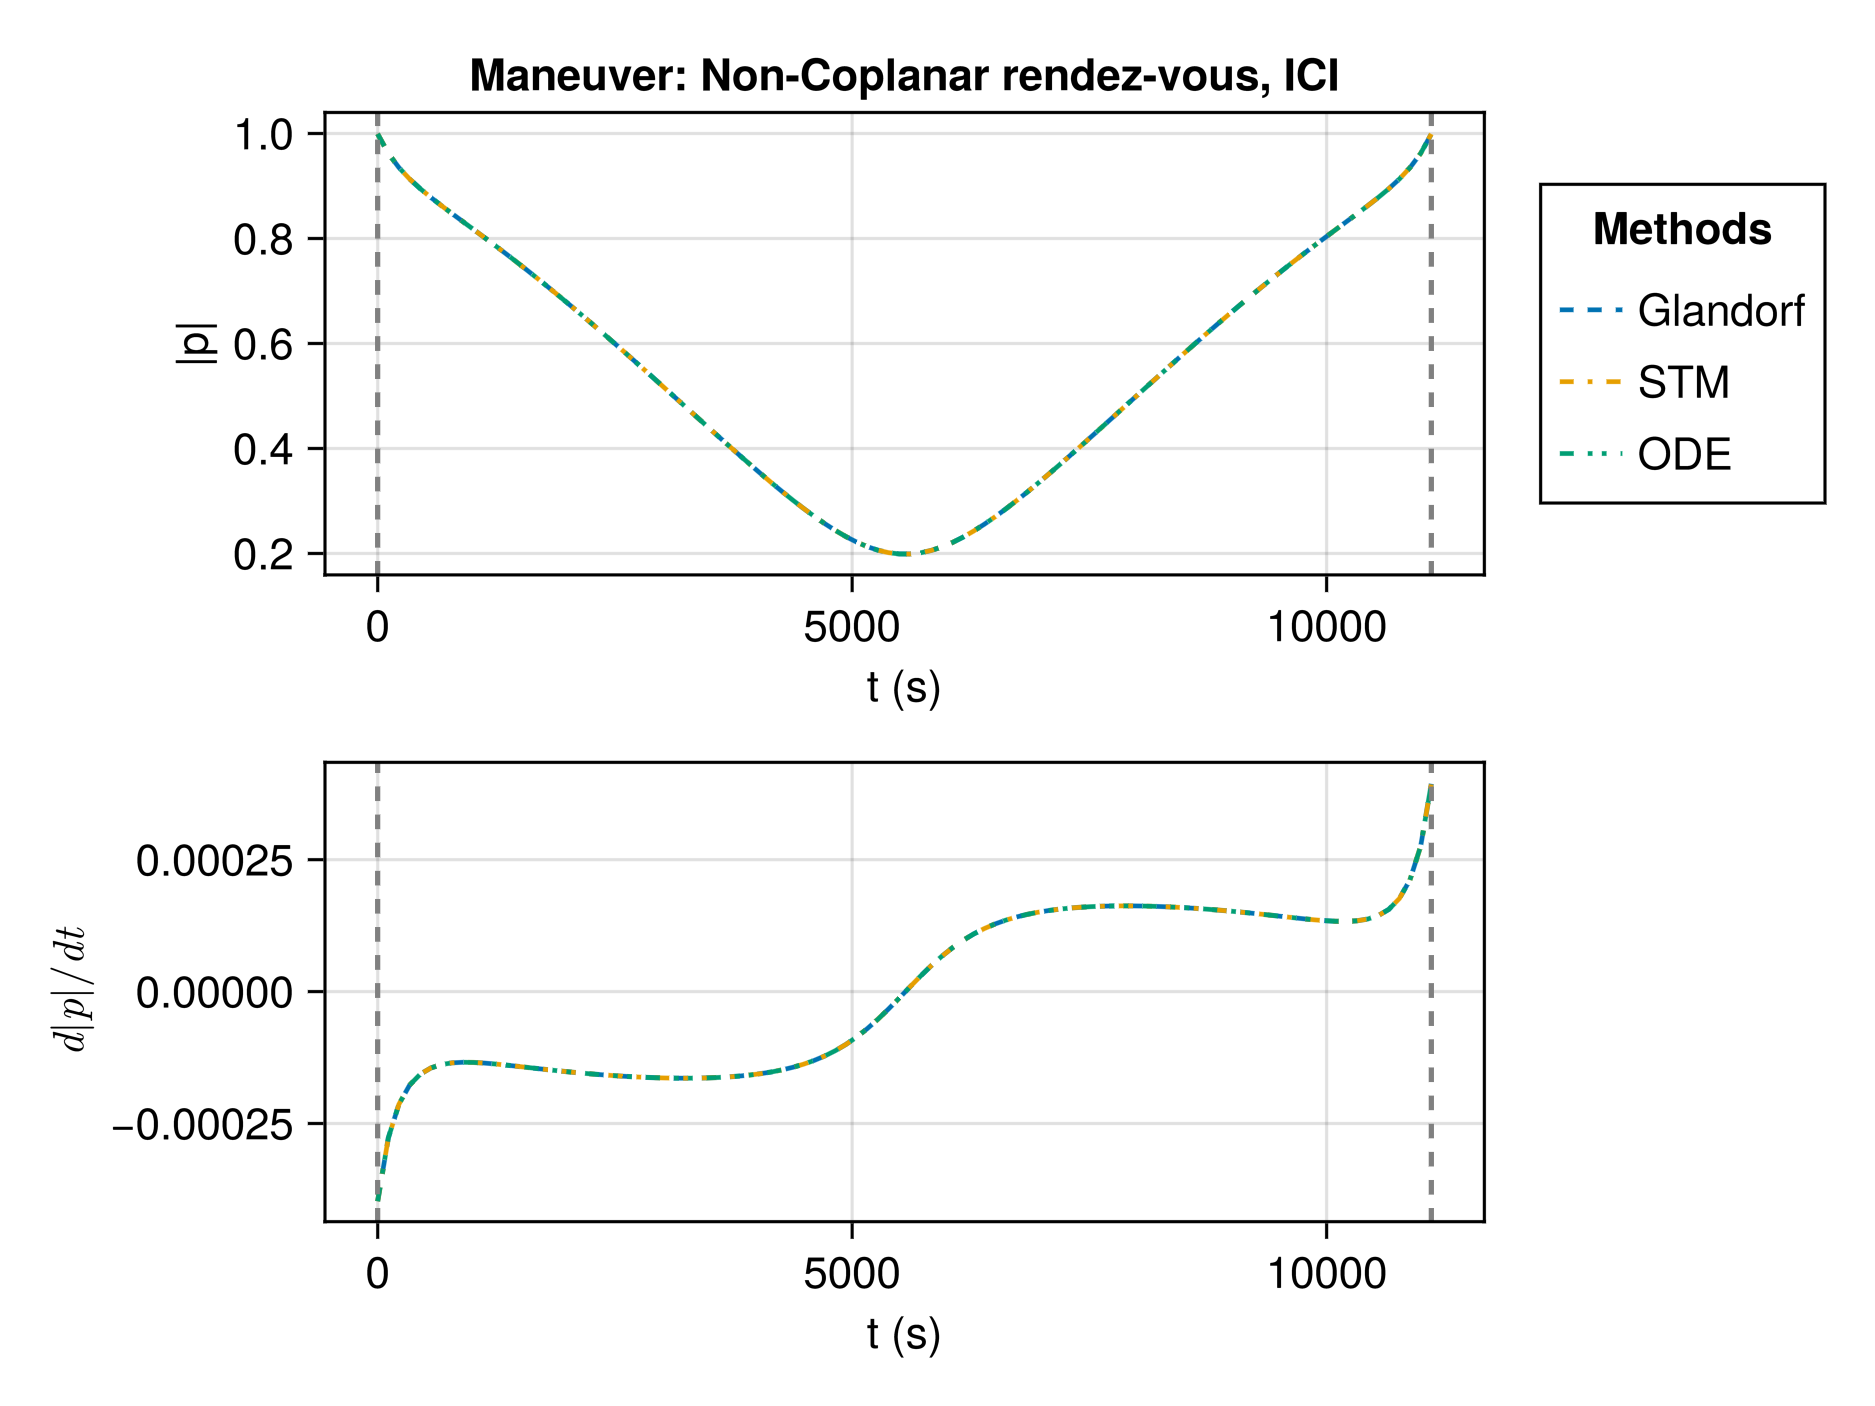
\includegraphics[width=\linewidth]{../results/two_body/ipv_noncop/ICI_primer_vector.png}
    \caption{Primer vector trajectory for two body noncoplanar \texttt{ICI} rendez-vous.}
    \label{fig:tb_ncop_ICI_pv}
\end{figure}

\begin{figure}[htbp]
    \centering
    \begin{subfigure}{0.49\linewidth}
        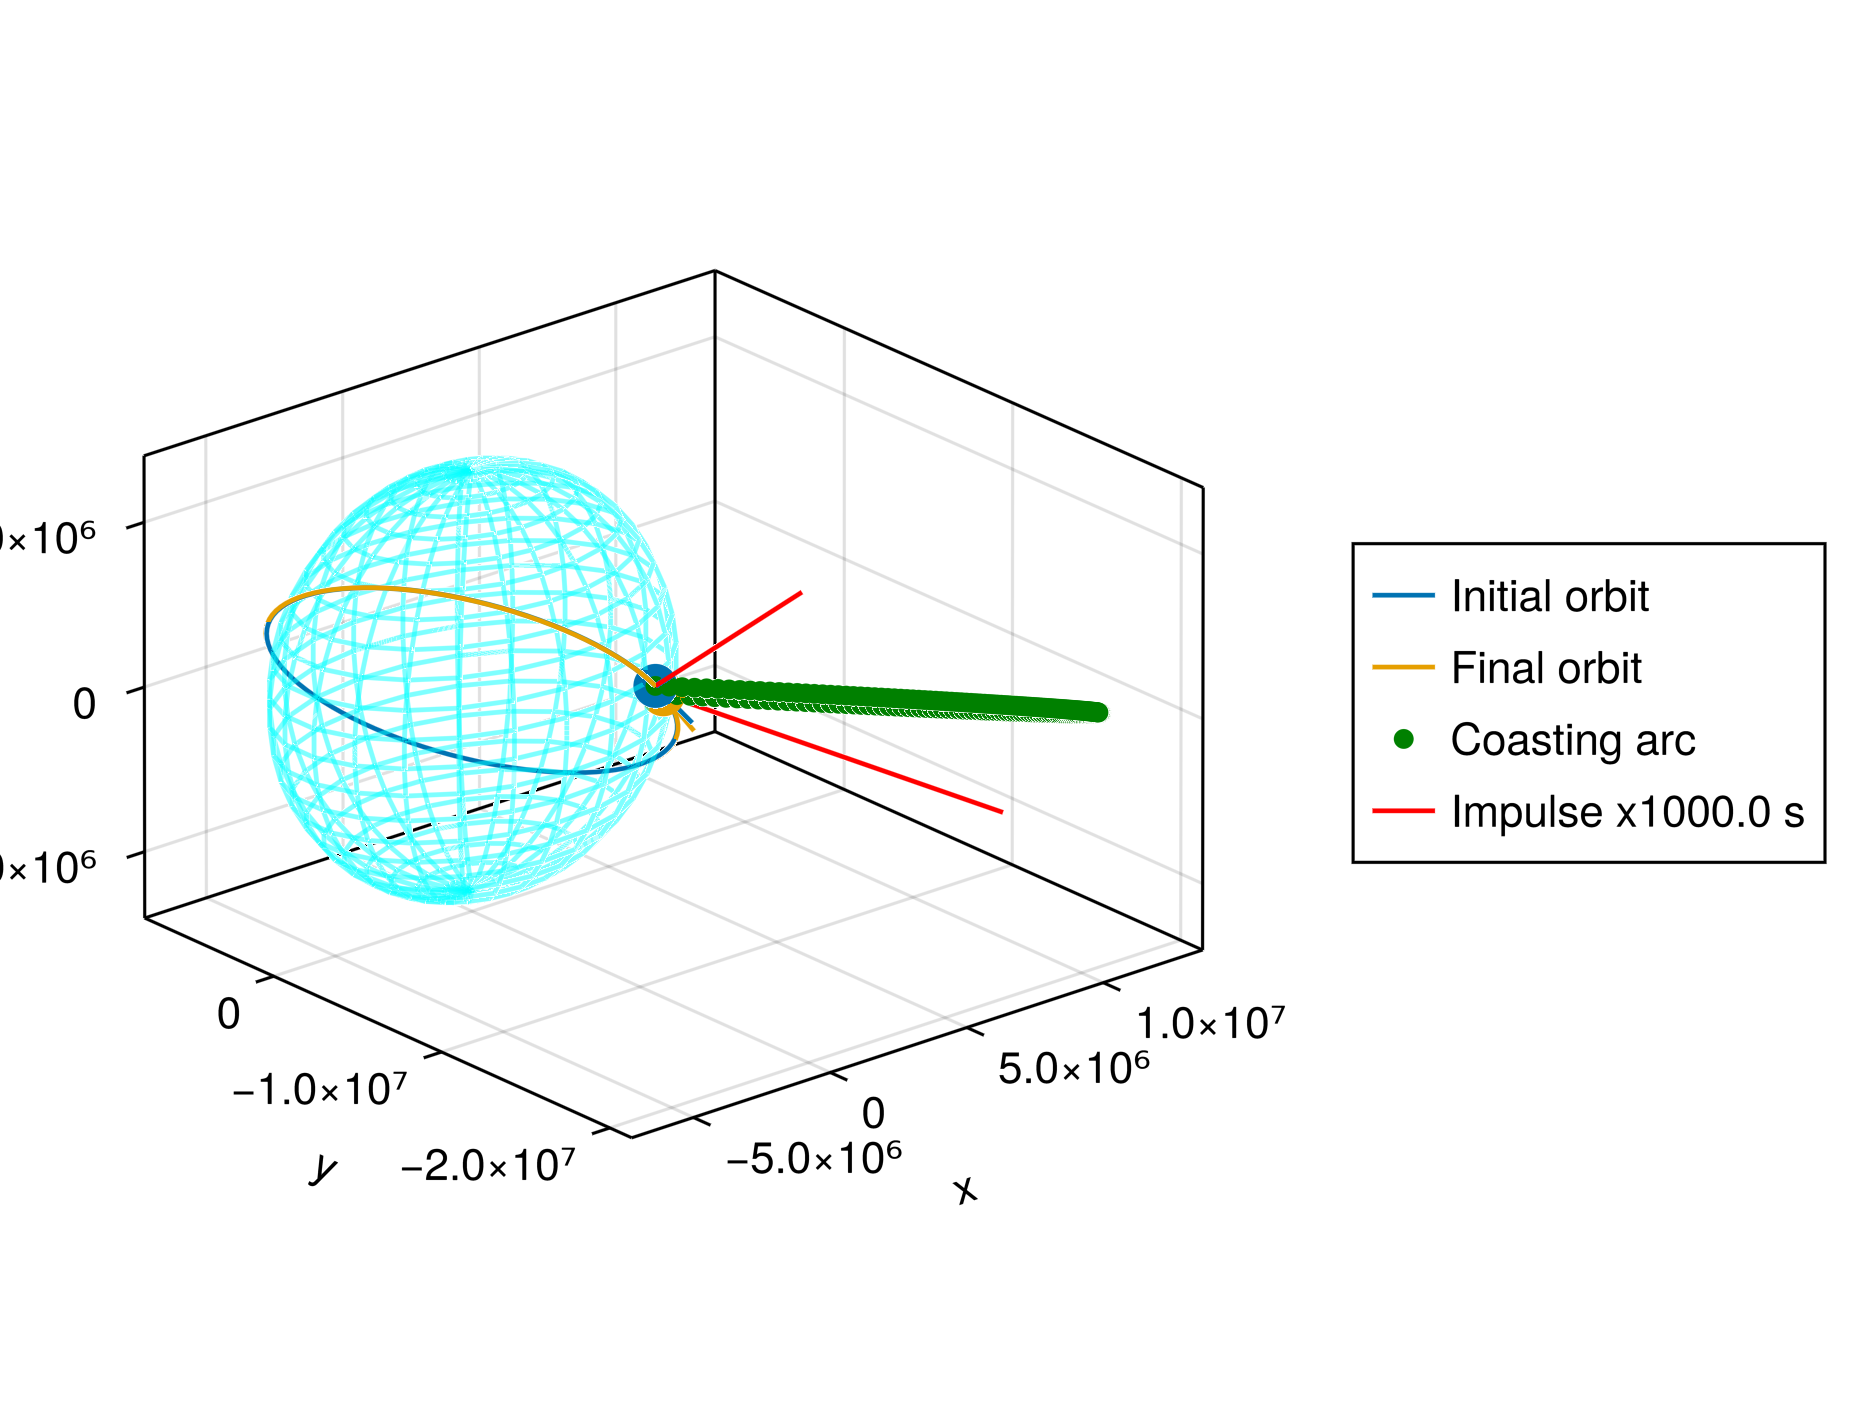
\includegraphics[width=\linewidth]{../results/two_body/ipv_noncop/ICI_3d.png}
        \caption{3D view.}
    \end{subfigure}
    \begin{subfigure}{0.49\linewidth}
        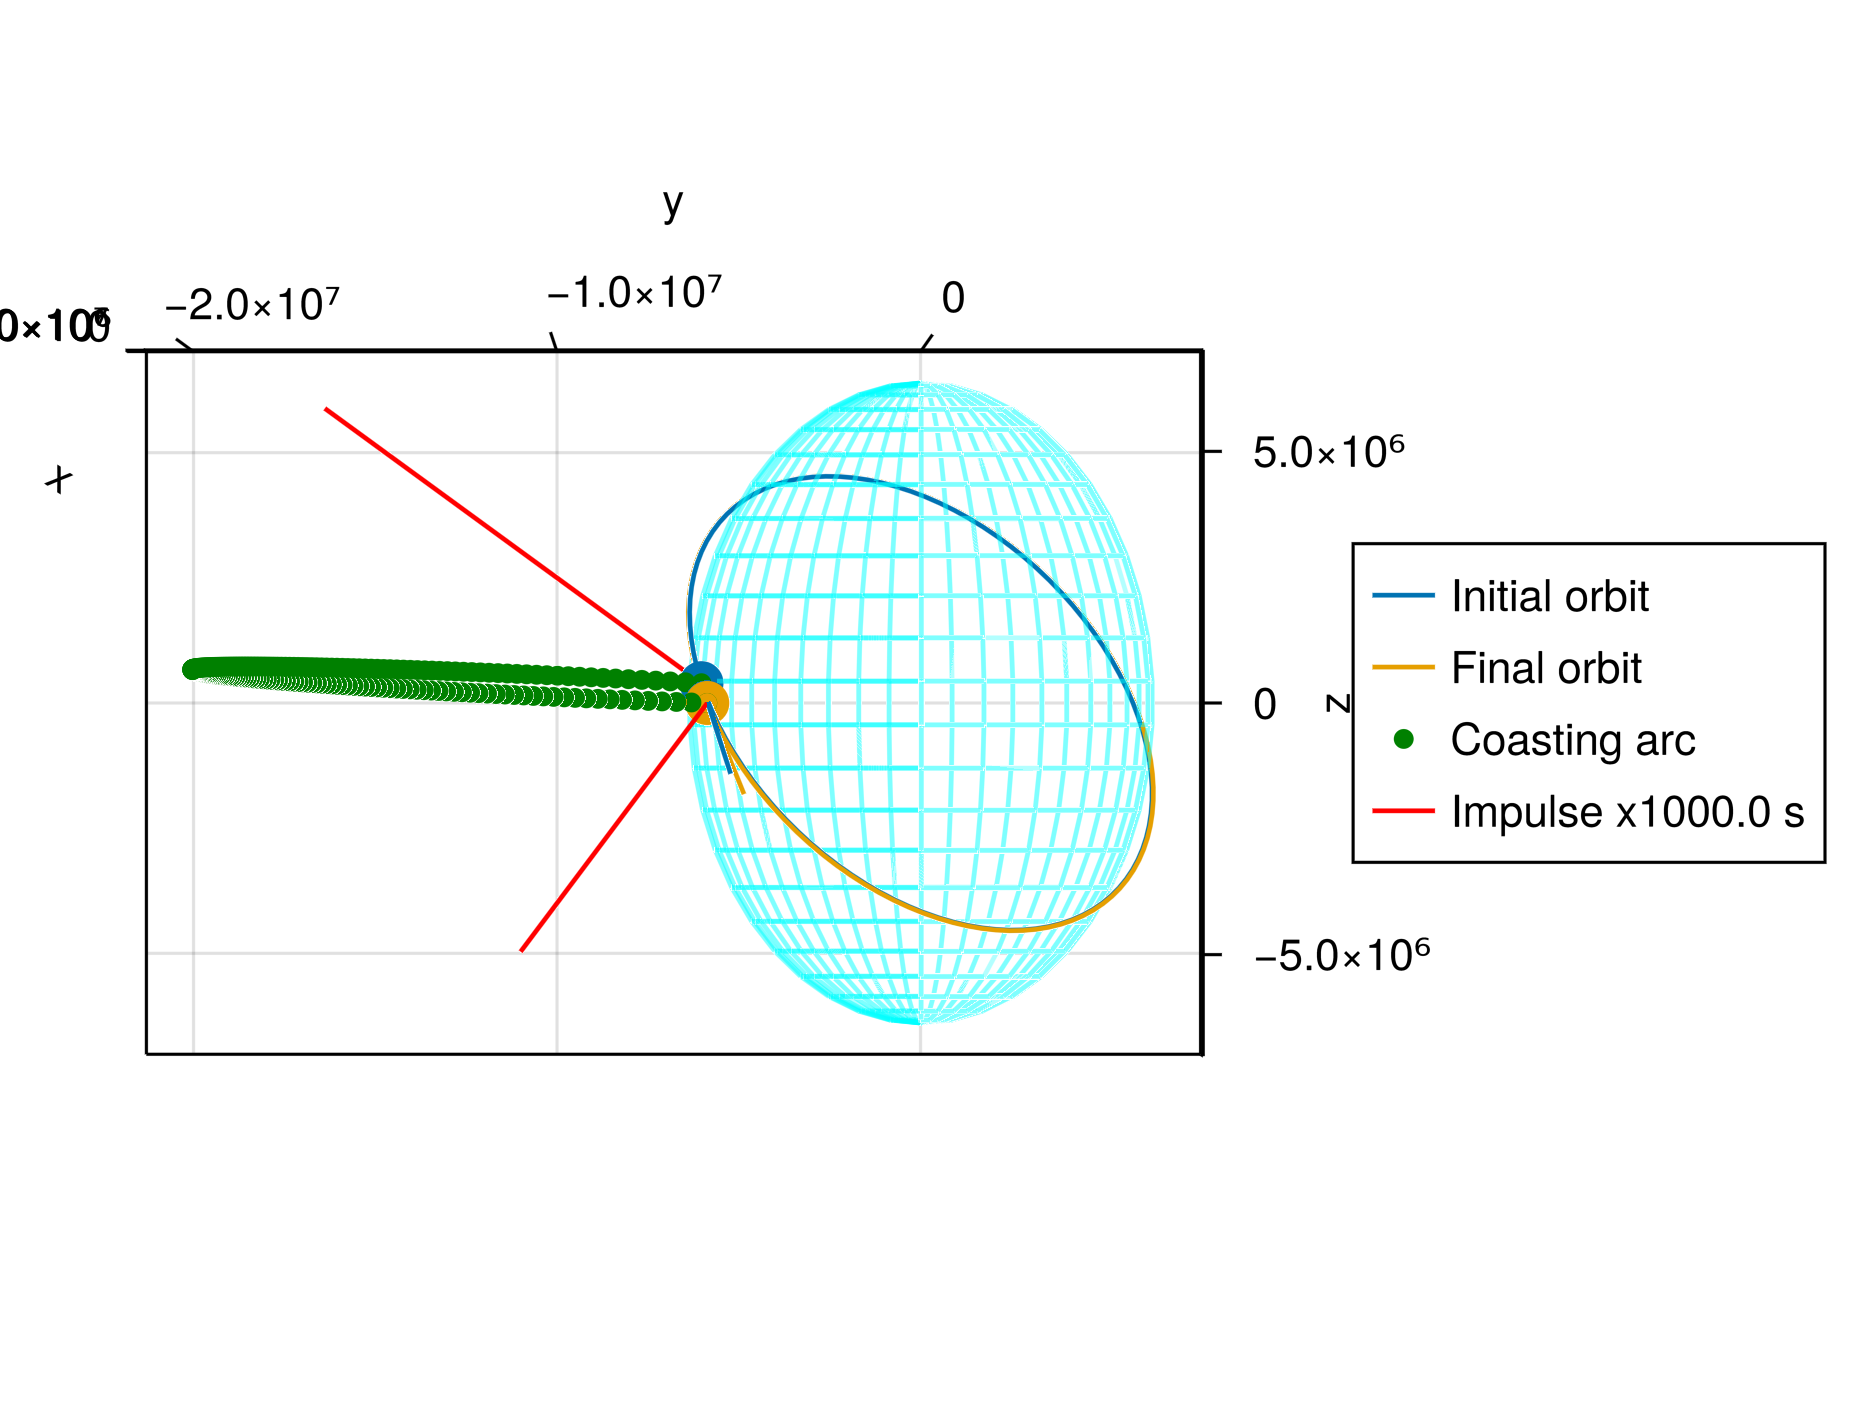
\includegraphics[width=\linewidth]{../results/two_body/ipv_noncop/ICI_x+.png}
        \caption{View from x+ axis.}
    \end{subfigure}
    \begin{subfigure}{0.49\linewidth}
        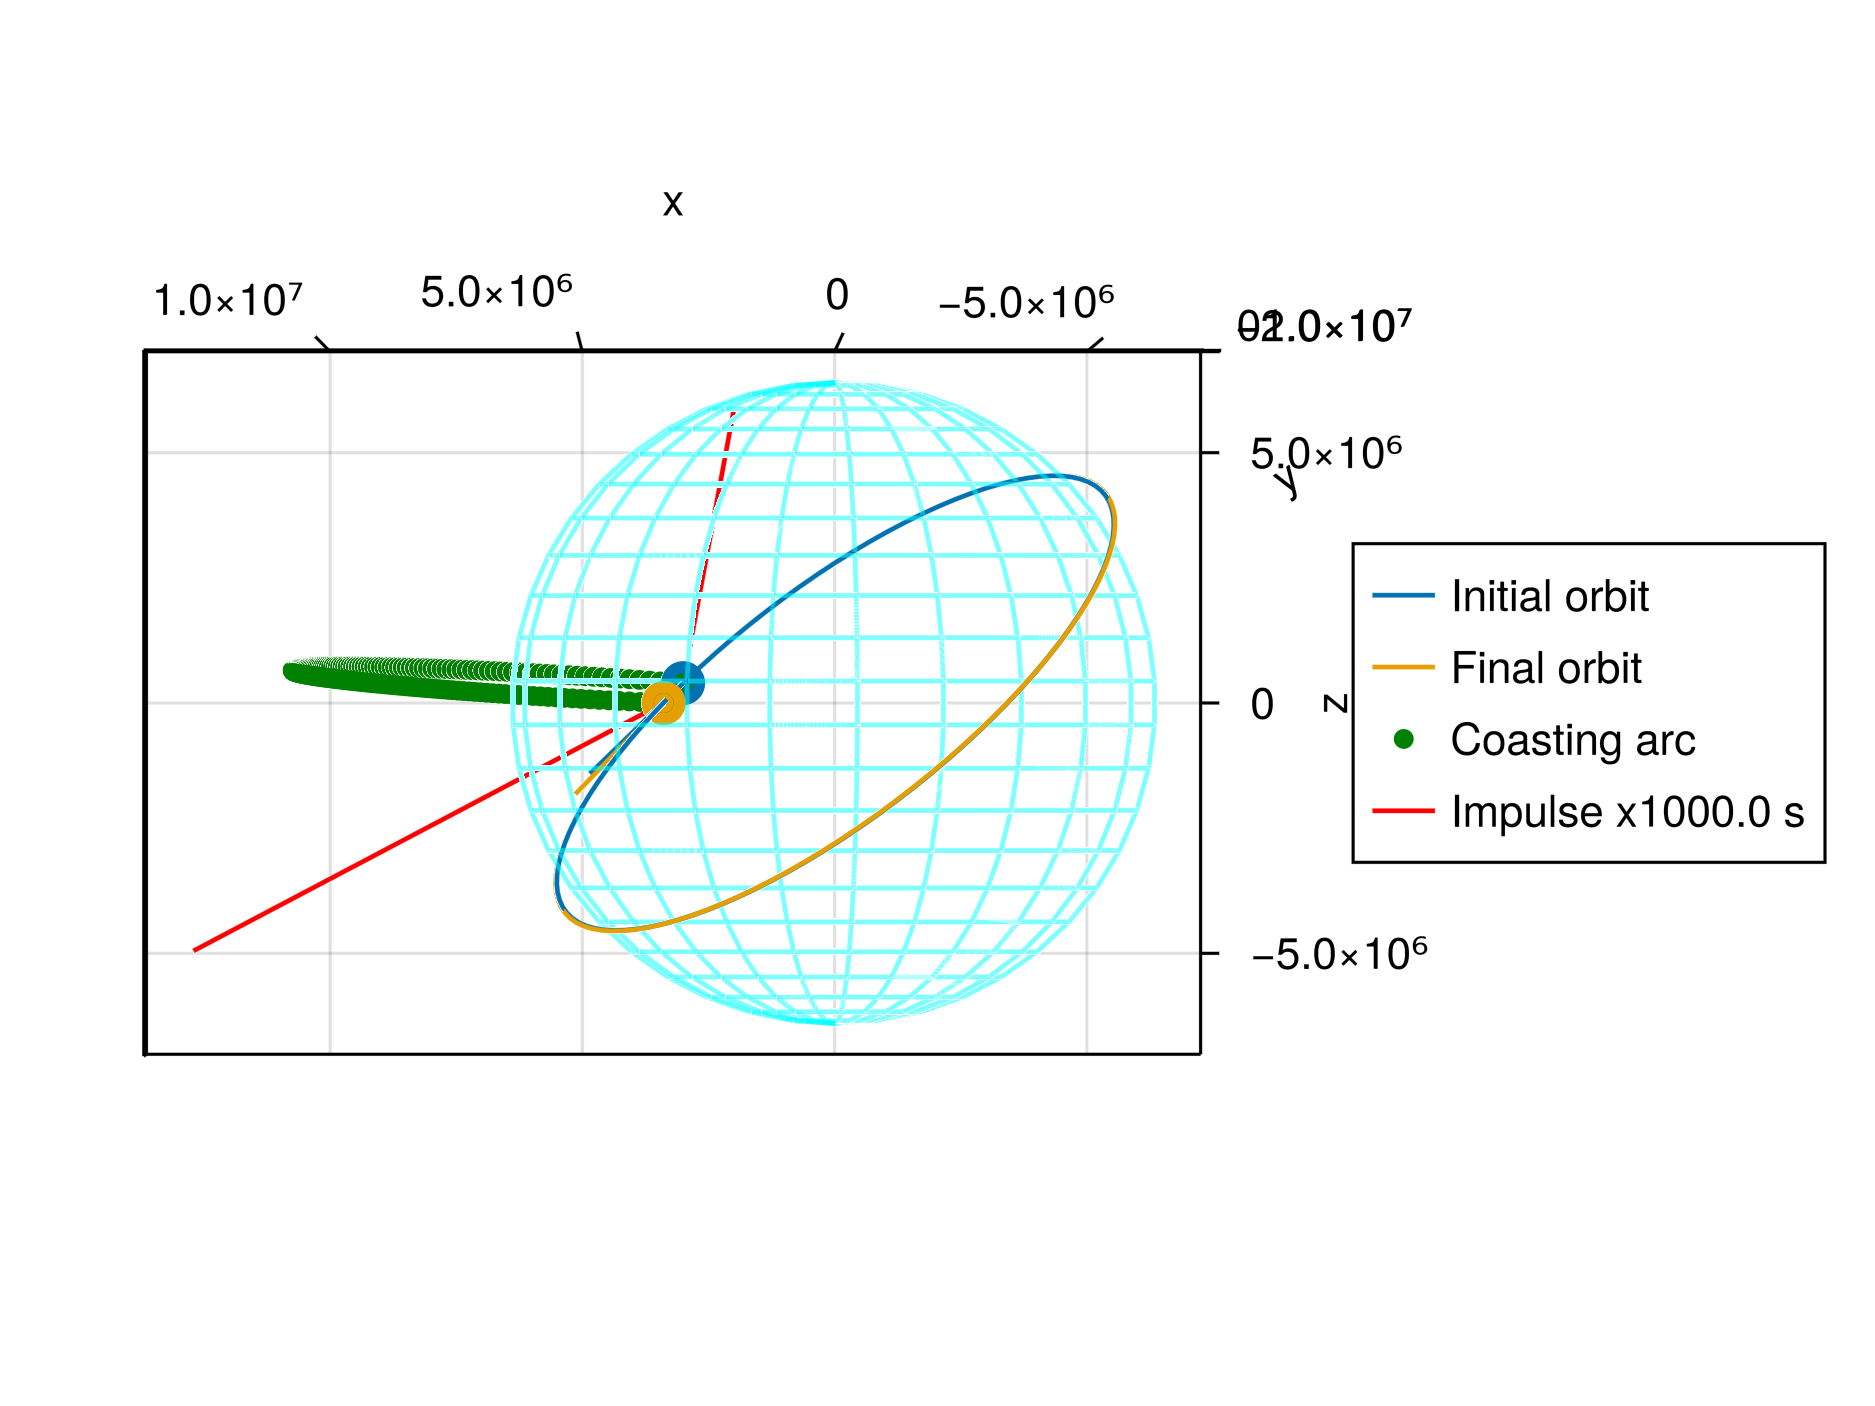
\includegraphics[width=\linewidth]{../results/two_body/ipv_noncop/ICI_y+.png}
        \caption{View from y+ axis.}
    \end{subfigure}
    \begin{subfigure}{0.49\linewidth}
        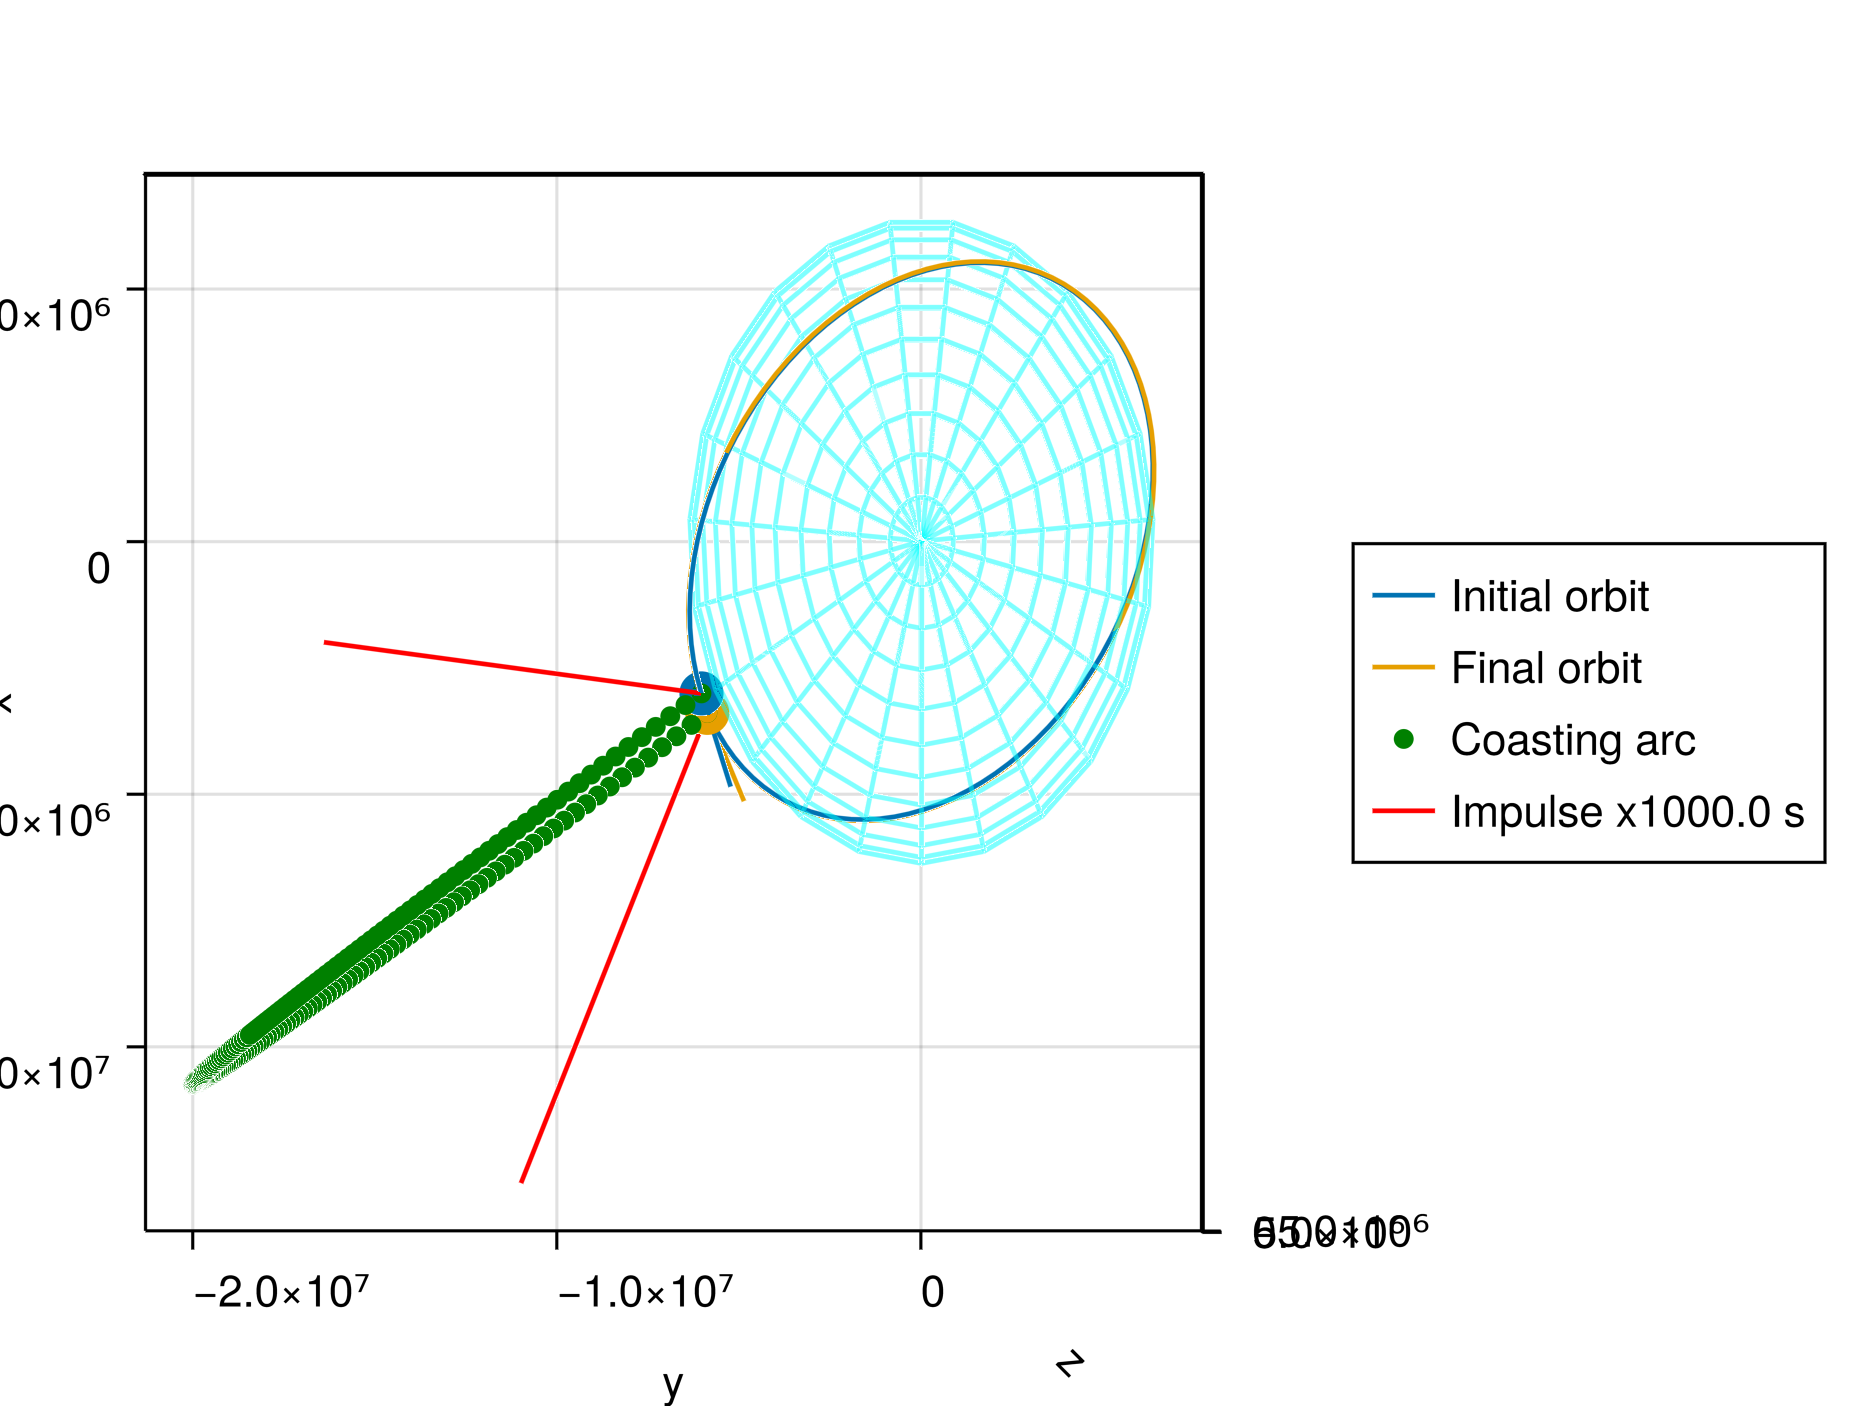
\includegraphics[width=\linewidth]{../results/two_body/ipv_noncop/ICI_z+.png}
        \caption{View from z+ axis.}
    \end{subfigure}
    \caption{Noncoplanar rendez-vous \texttt{ICI} maneuver 3D view and projections}
    \label{fig:tb_ncop_ICI_figs}
\end{figure}

Therefore, a \texttt{CICIC} maneuver case was optimized next. The maneuver's summary, primer vector trajectory, and spatial views can be seen in Table~\ref{tab:tb_ncop_CICIC_tab}, Figure~\ref{fig:tb_ncop_CICIC_pv} and Figure~\ref{fig:tb_ncop_CICIC_figs}. Now, the cost is much lower, and the trajectory is very close to the natural orbit of the satellite. However, the primer vector history violates the norm condition and shows that the addition of an extra impulse can lower the cost even further. 

\begin{table}[htpb]
    \centering
    \begin{tabular}{cccc} \toprule
    \multicolumn{2}{c}{\textbf{Maneuver type}} & \multicolumn{2}{c}{CICIC} \\ \midrule
    \(L\) (m) & \(T\) (s) & \(\varepsilon\) & \(\Delta x_{f}\) (m)    \\ \midrule
    6.7631e6          & 11107.158          & 1.00e-06                & 0.0                        \\ \midrule
    \(\max \lVert p \rVert\) & 3.327     & \textbf{Diagnostic}   & Add impulse        \\ \midrule
    \textbf{Impulse} & \(t\) (s) & \(\Delta v\) (m/s) & \(1 - p \cdot \hat{u}\) \\ \midrule
    1                 & 6644.30733          & 37.29252             & -0.0                    \\
    2                 & 10689.86179          & 16.20984             & -0.0                    \\\midrule
    \textbf{Total}   & 11107.1576          & 53.50237             &                     \\ \bottomrule   
    \end{tabular}
    \caption{Summary of optimization for two body noncoplanar \texttt{CICIC} rendez-vous.}
    \label{tab:tb_ncop_CICIC_tab}
\end{table}

\begin{figure}[htbp]
    \centering
    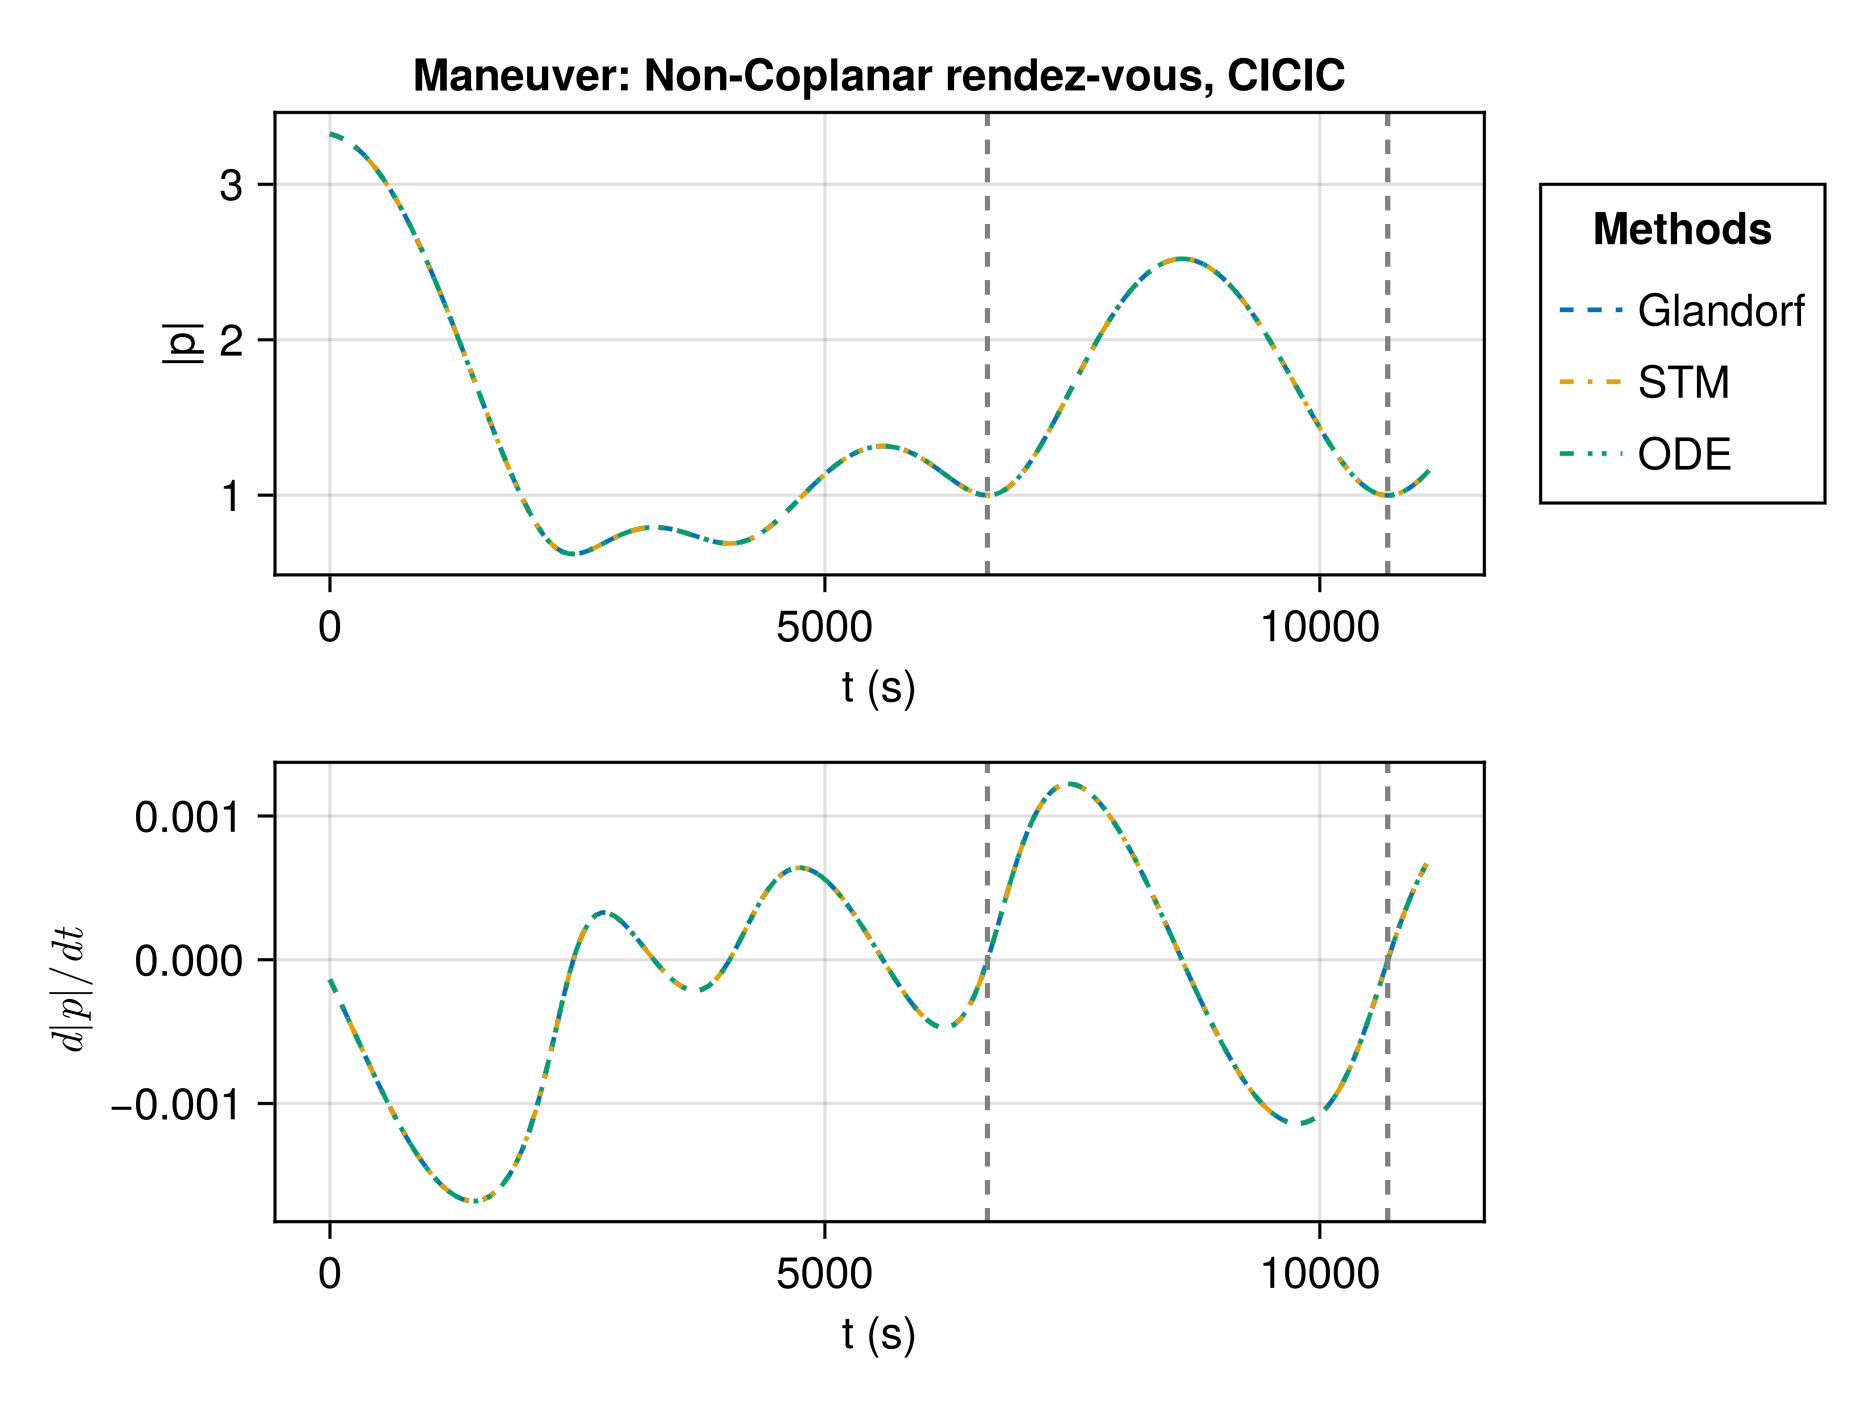
\includegraphics[width=\linewidth]{../results/two_body/ipv_noncop/CICIC_primer_vector.png}
    \caption{Primer vector trajectory for two body noncoplanar \texttt{CICIC} rendez-vous.}
    \label{fig:tb_ncop_CICIC_pv}
\end{figure}

\begin{figure}[htbp]
    \centering
    \begin{subfigure}{0.49\linewidth}
        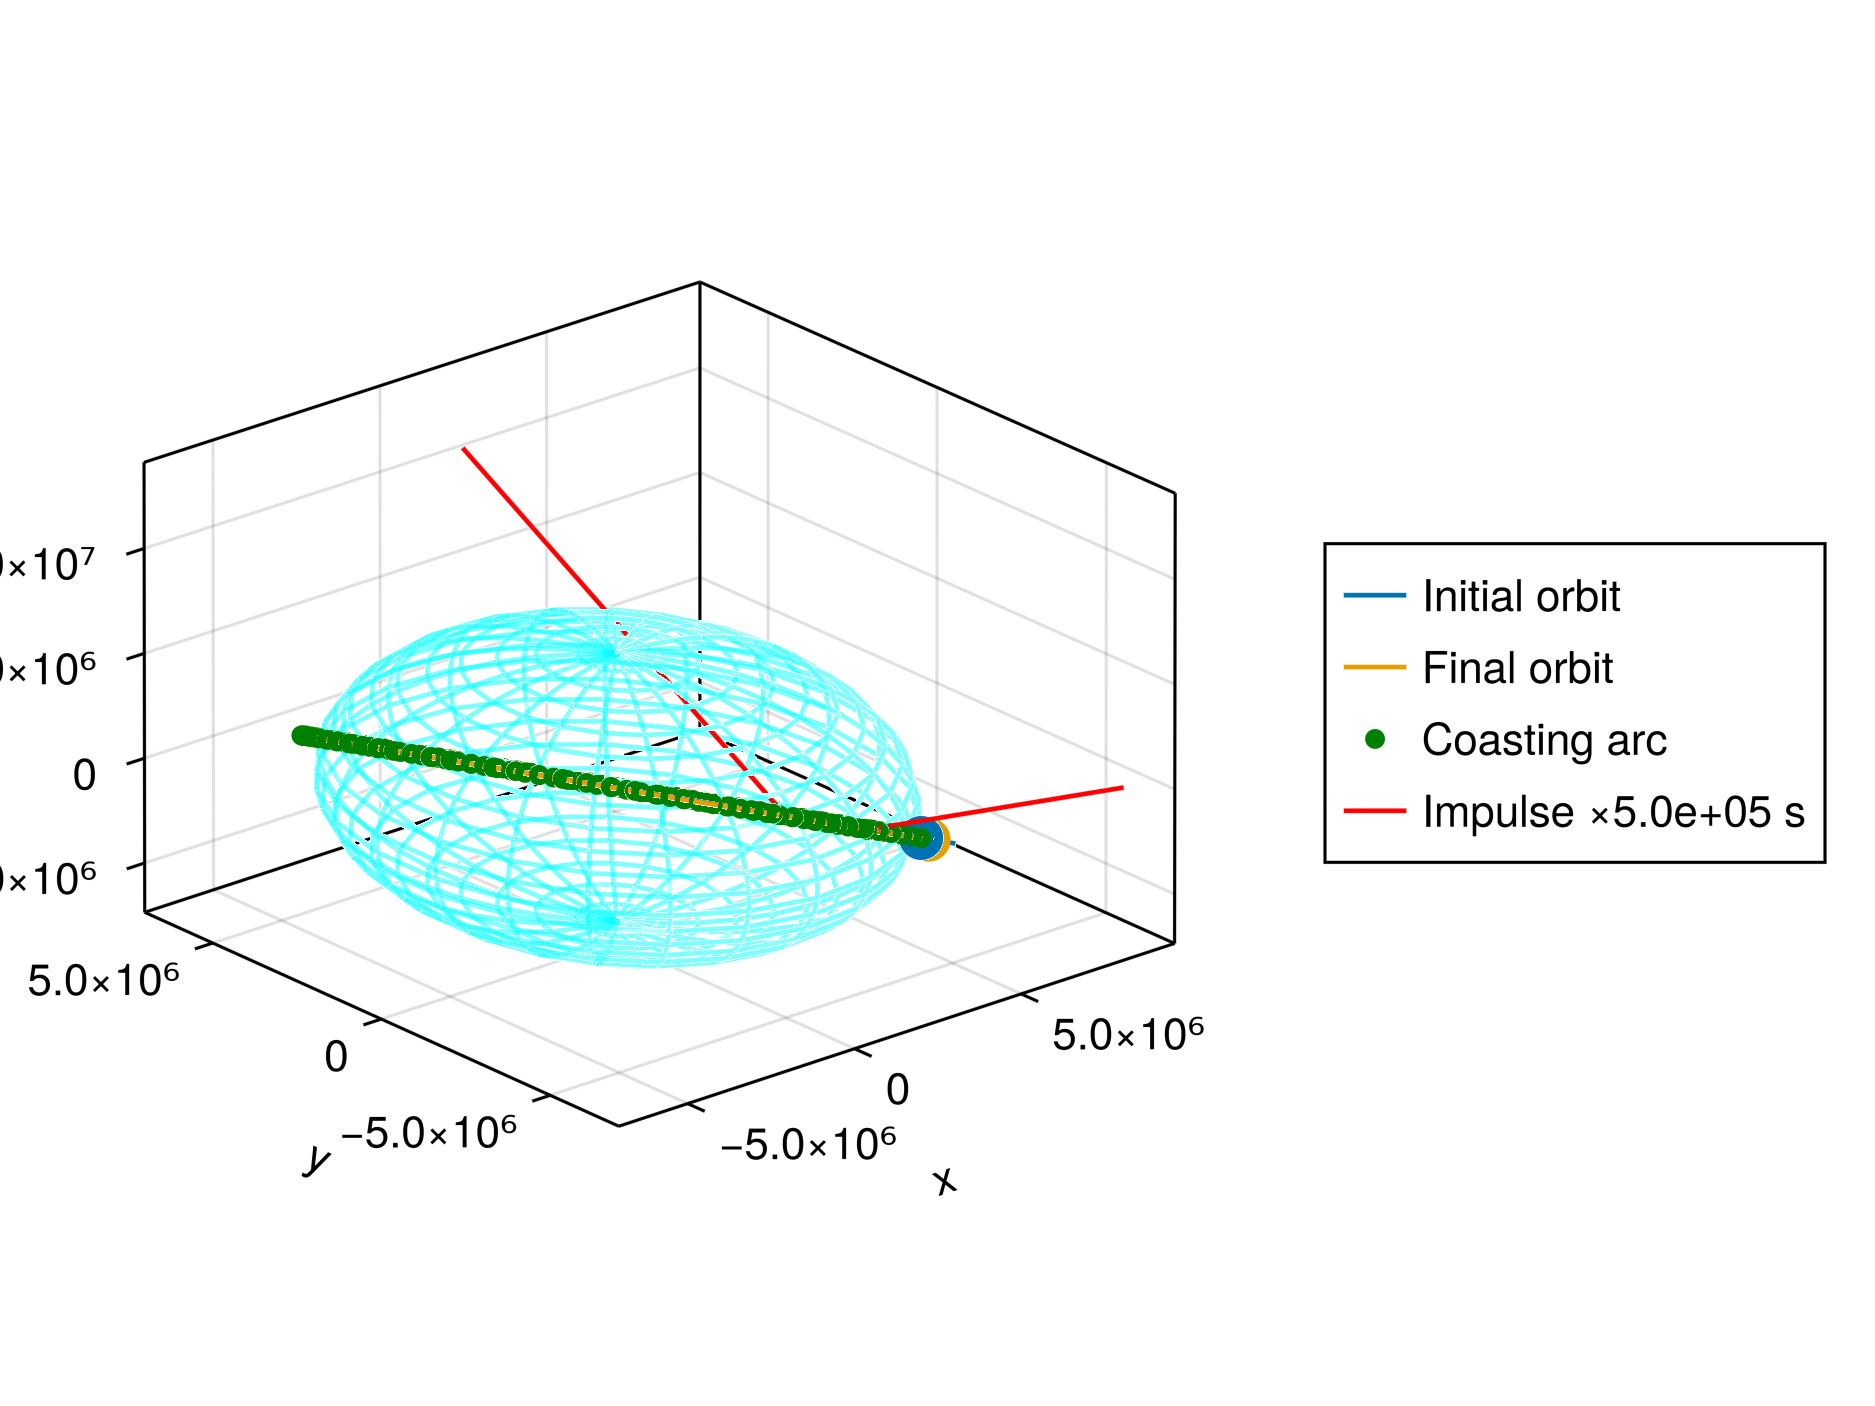
\includegraphics[width=\linewidth]{../results/two_body/ipv_noncop/CICIC_3d.png}
        \caption{3D view.}
    \end{subfigure}
    \begin{subfigure}{0.49\linewidth}
        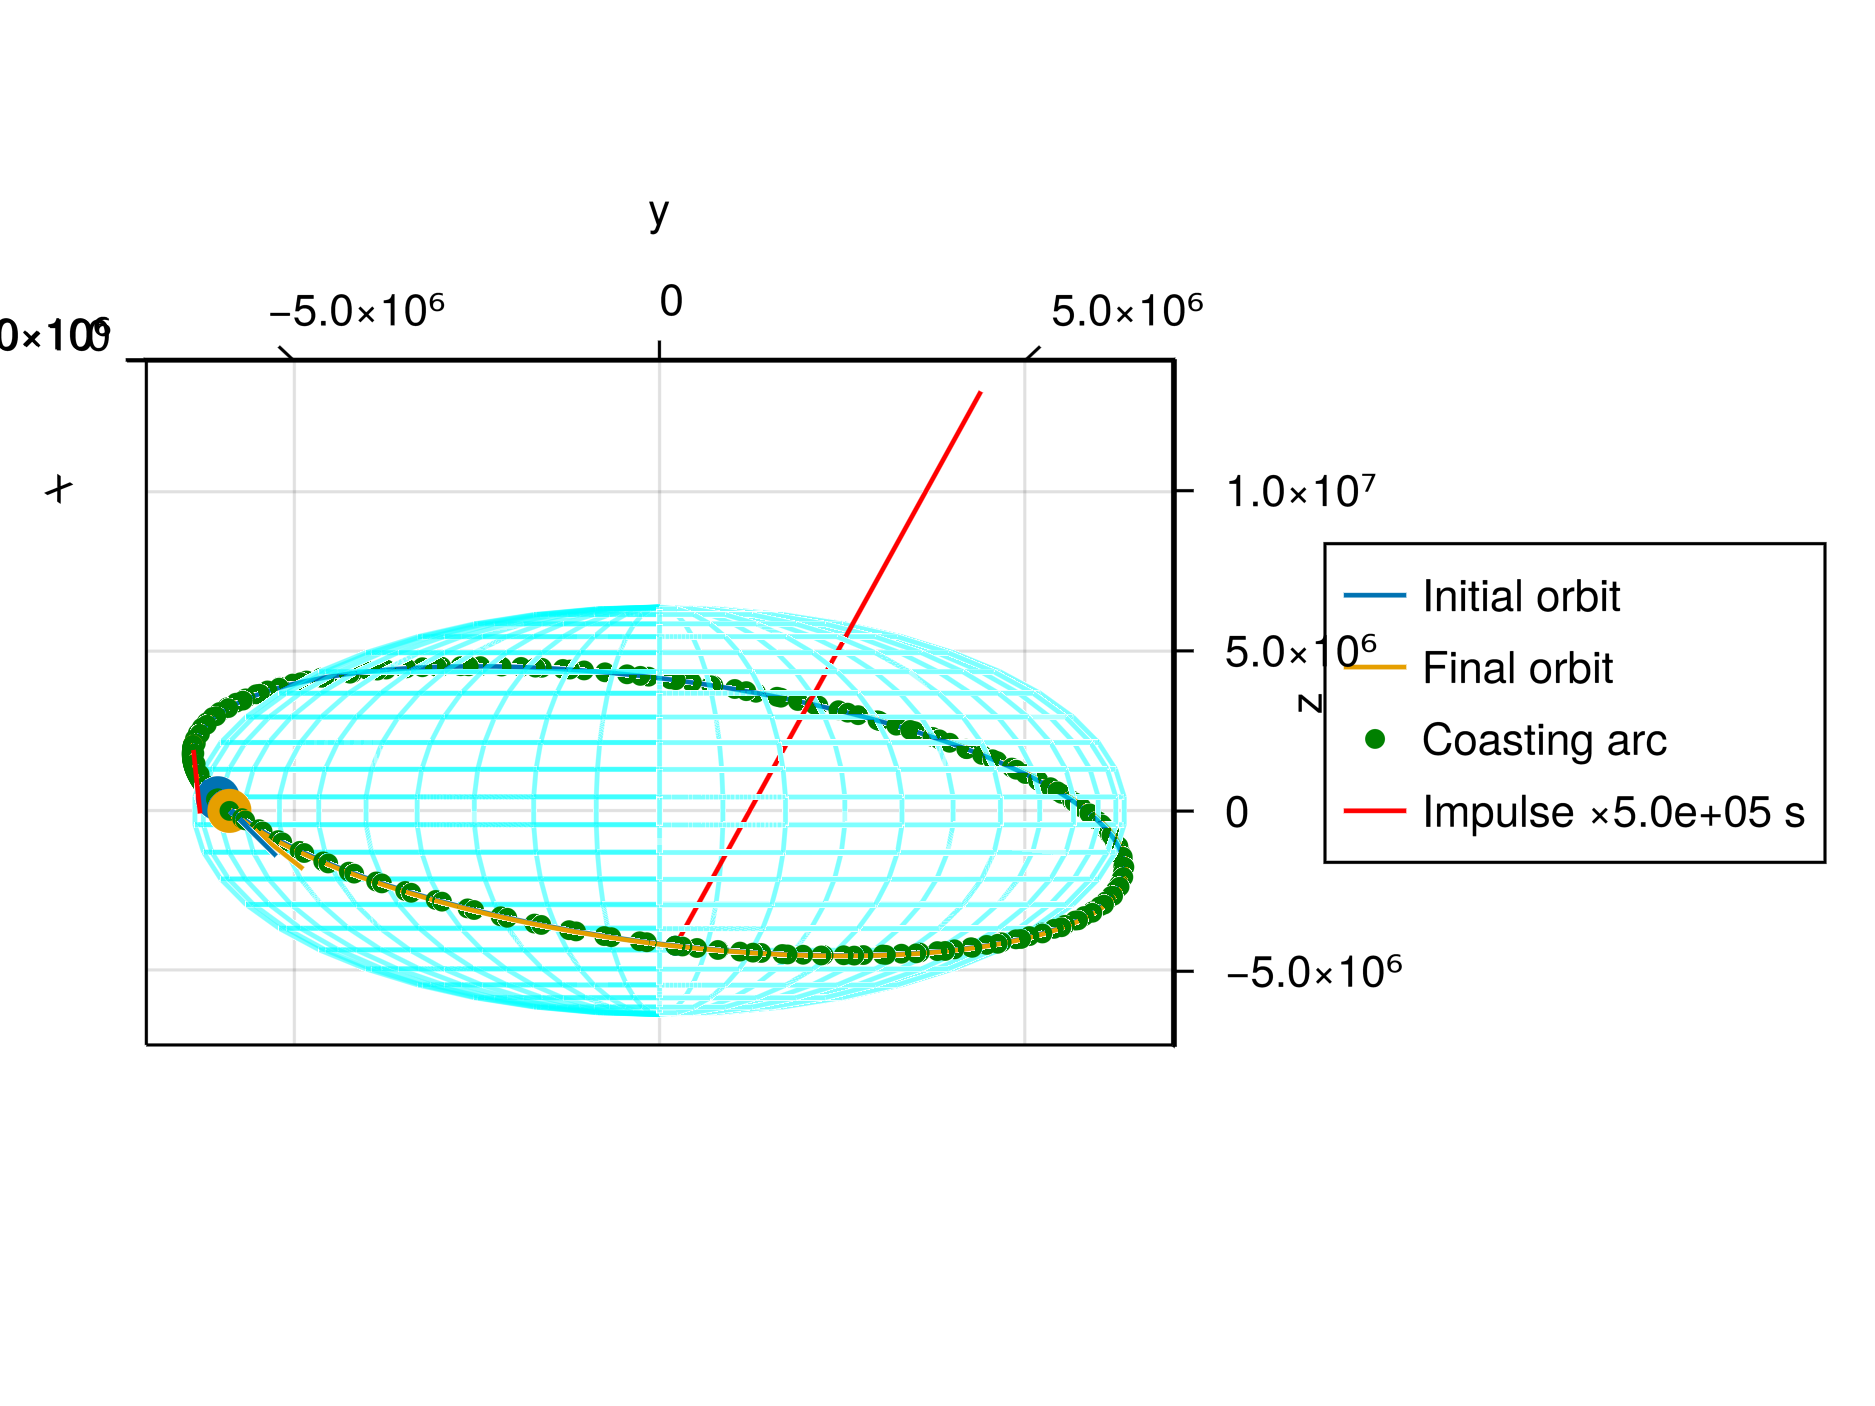
\includegraphics[width=\linewidth]{../results/two_body/ipv_noncop/CICIC_x+.png}
        \caption{View from x+ axis.}
    \end{subfigure}
    \begin{subfigure}{0.49\linewidth}
        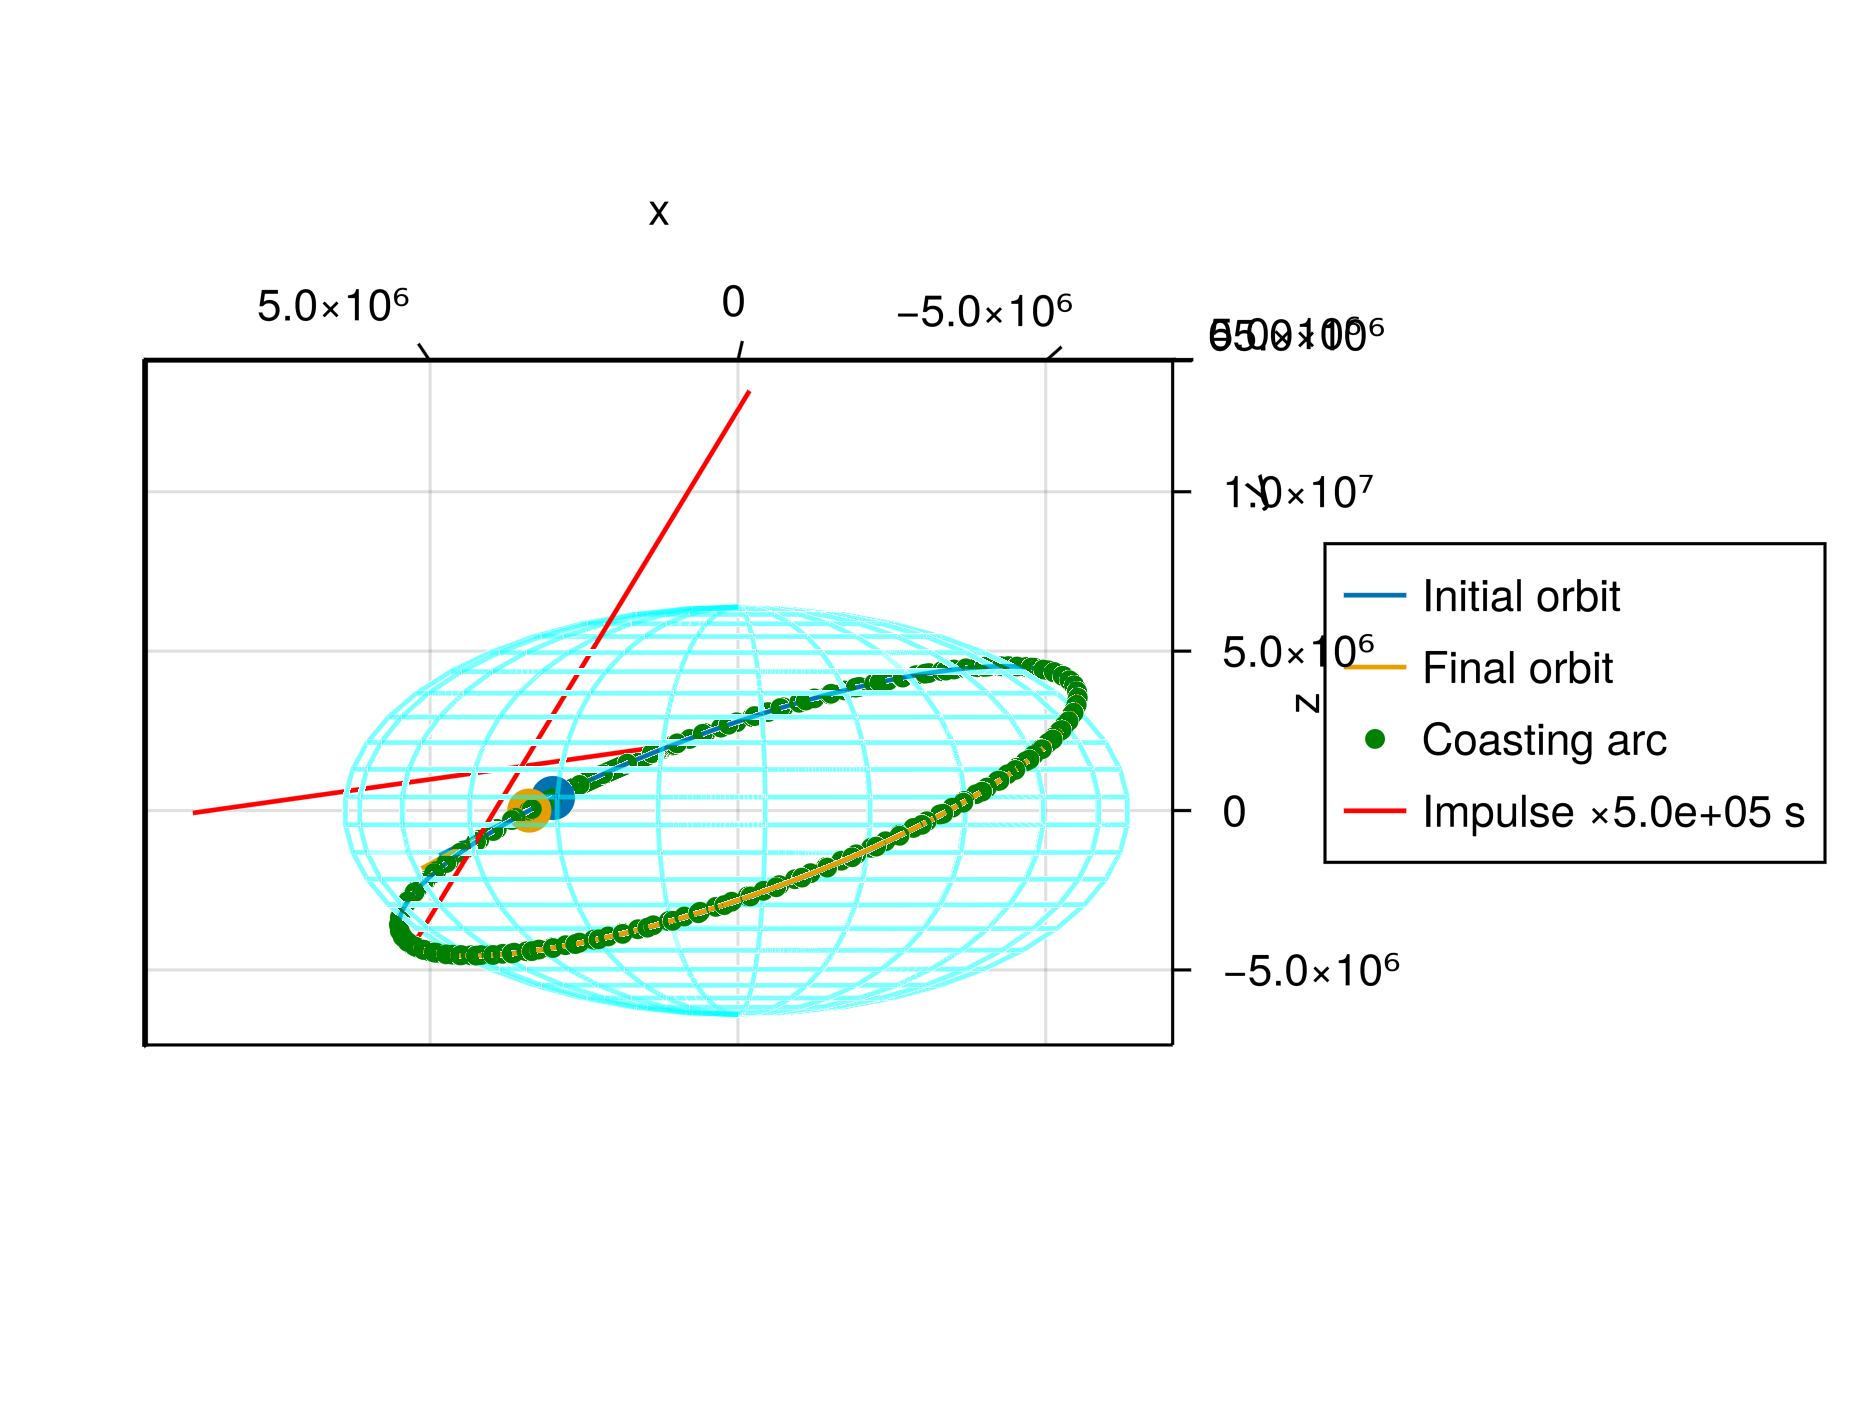
\includegraphics[width=\linewidth]{../results/two_body/ipv_noncop/CICIC_y+.png}
        \caption{View from y+ axis.}
    \end{subfigure}
    \begin{subfigure}{0.49\linewidth}
        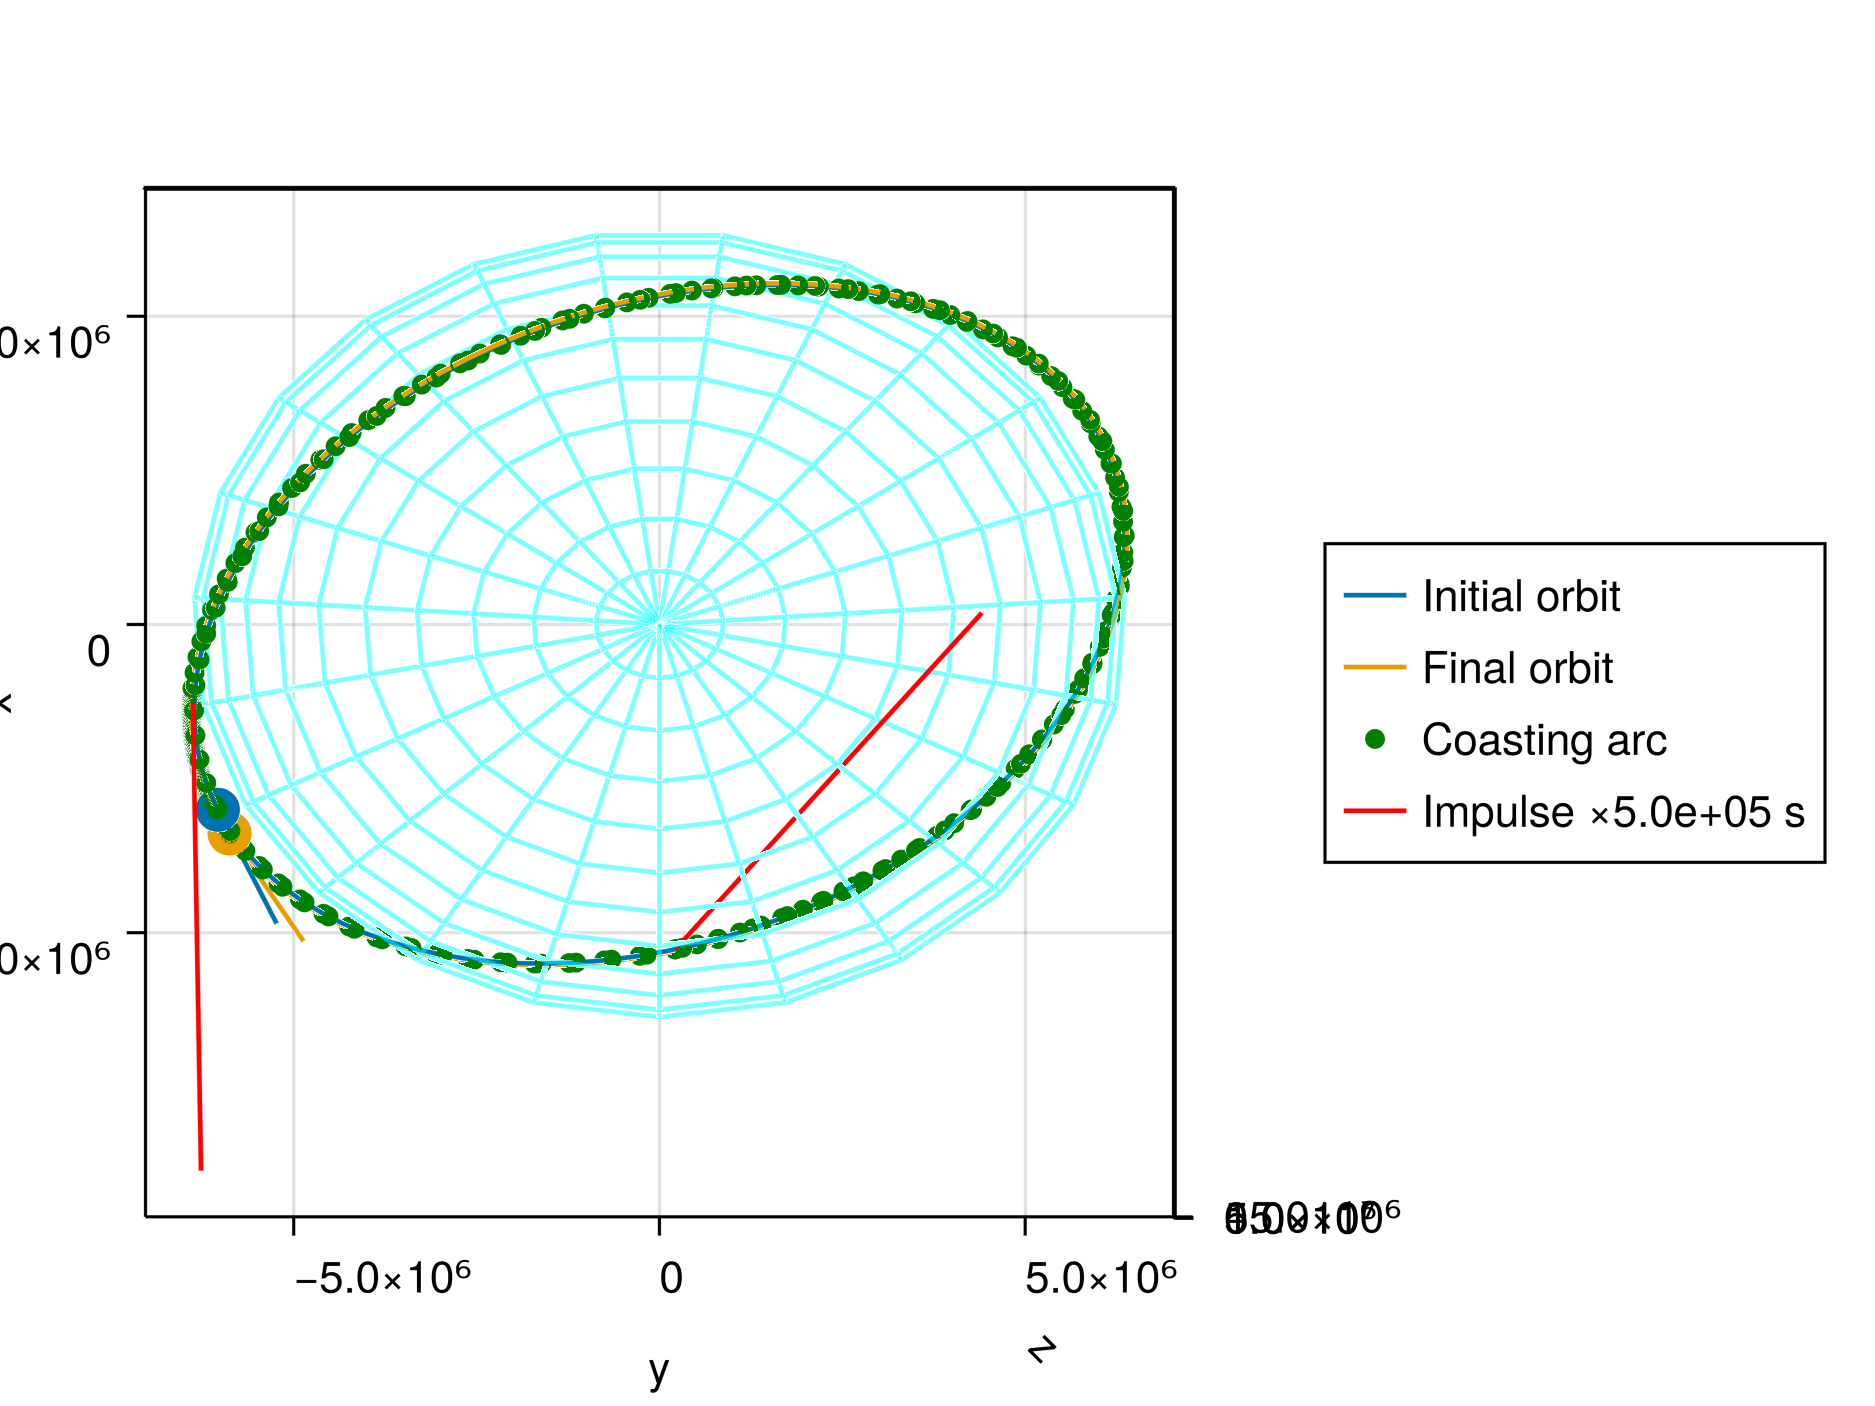
\includegraphics[width=\linewidth]{../results/two_body/ipv_noncop/CICIC_z+.png}
        \caption{View from z+ axis.}
    \end{subfigure}
    \caption{Noncoplanar rendez-vous \texttt{CICIC} maneuver 3D view and projections}
    \label{fig:tb_ncop_CICIC_figs}
\end{figure}

A \texttt{CICICIC} maneuver was searched based on the previous results. The spatial view is omitted since the trajectory closely resembles the natural orbit of the satellite. The maneuver summary and primer vector history are shown in Table~\ref{tab:tb_ncop_CICICIC_tab} and Figure~\ref{fig:tb_ncop_CICICIC_pv}. The addition of yet another impulse did reduce the \(\Delta v\) cost, but not as dramatically as the addition of initial and final coasts. Again, the maximum primer vector norm exceeds unity, which suggests another addition of impulse.

\begin{table}[htpb]
    \centering
    \begin{tabular}{cccc} \toprule
    \multicolumn{2}{c}{\textbf{Maneuver type}} & \multicolumn{2}{c}{CICICIC} \\ \midrule
    \(L\) (m) & \(T\) (s) & \(\varepsilon\) & \(\Delta x_{f}\) (m)    \\ \midrule
    6.7631e6          & 11107.158          & 1.00e-05                & 0.0                        \\ \midrule
    \(\max \lVert p \rVert\) & 1.9638     & \textbf{Diagnostic}   & Add impulse        \\ \midrule
    \textbf{Impulse} & \(t\) (s) & \(\Delta v\) (m/s) & \(1 - p \cdot \hat{u}\) \\ \midrule
    1                 & 3370.1071          & 11.76294             & -0.0                    \\
    2                 & 6774.61652          & 10.56494             & 0.0                    \\
    3                 & 9176.42663          & 20.74554             & -0.0                    \\\midrule
    \textbf{Total}   & 11107.1576          & 43.07342             &                     \\ \bottomrule   
    \end{tabular}
    \caption{Summary of optimization for two body noncoplanar \texttt{CICICIC} rendez-vous.}
    \label{tab:tb_ncop_CICICIC_tab}
\end{table}

\begin{figure}[htbp]
    \centering
    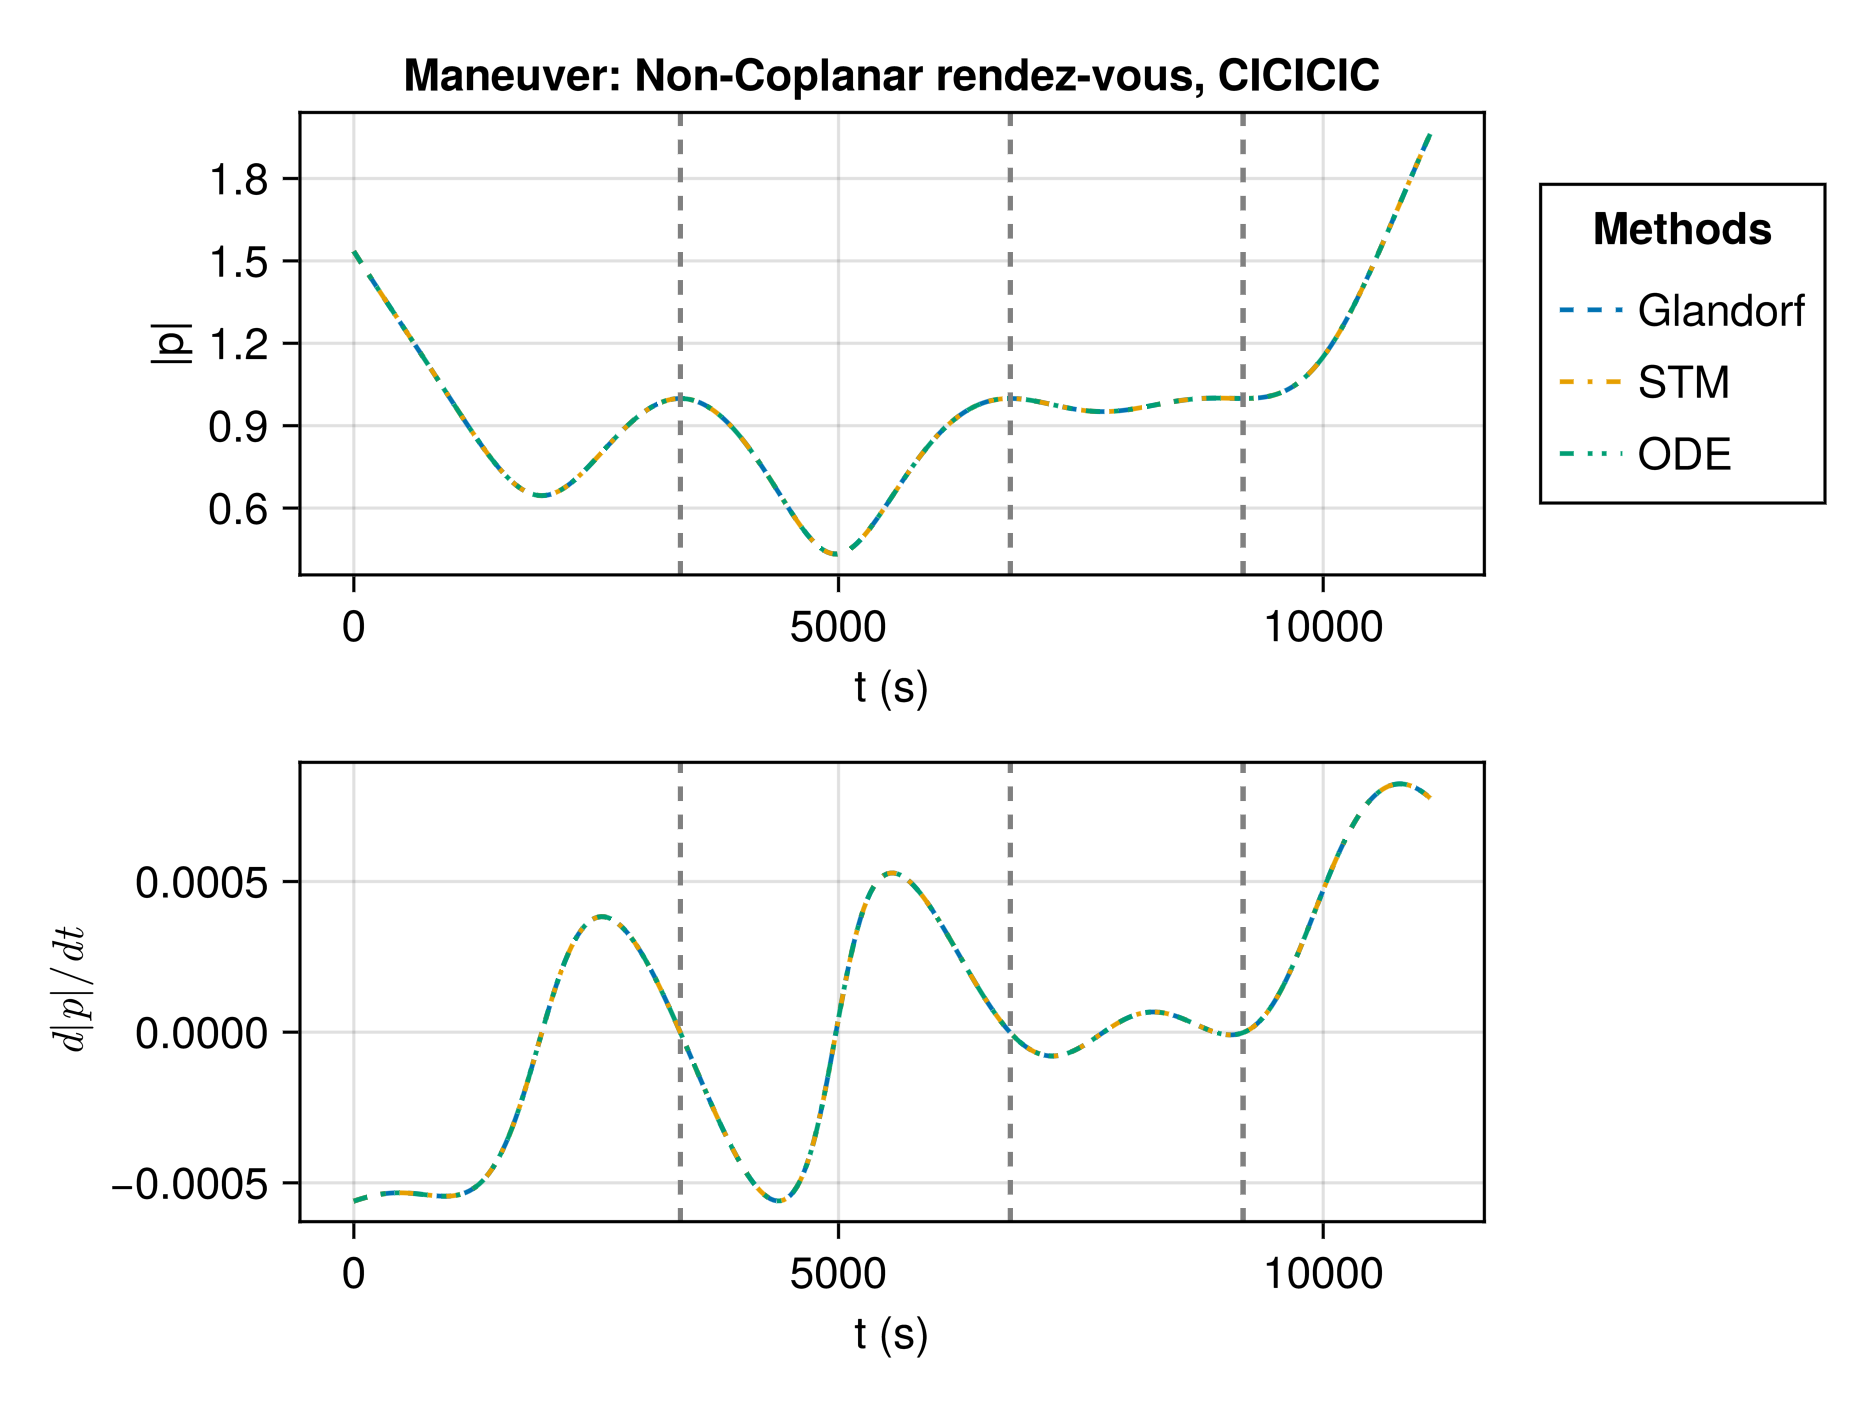
\includegraphics[width=\linewidth]{../results/two_body/ipv_noncop/CICICIC_primer_vector.png}
    \caption{Primer vector trajectory for two body noncoplanar \texttt{CICICIC} rendez-vous.}
    \label{fig:tb_ncop_CICICIC_pv}
\end{figure}

Finally, the addition of a fourth impulse attains the primer vector necessary conditions, as attested in its trajectory in Figure~\ref{fig:tb_ncop_CICICICIC_pv} and its summary in Table~\ref{tab:tb_ncop_CICICICIC_tab}. A small error of \(0.4\%\) has been allowed in the primer vector norm, which is small enough that only a very small fifth impulse would marginally reduce cost, for no tangible algorithmic gain. The final velocity cost is well within feasible for many spatial applications, with the caveat that the spacecraft must be correctly pointed at four points in time. 

\begin{table}[htpb]
    \centering
    \begin{tabular}{cccc} \toprule
    \multicolumn{2}{c}{\textbf{Maneuver type}} & \multicolumn{2}{c}{CICICICIC} \\ \midrule
    \(L\) (m) & \(T\) (s) & \(\varepsilon\) & \(\Delta x_{f}\) (m)    \\ \midrule
    6.7631e6          & 11107.158          & 1.00e-05                & 0.04983                        \\ \midrule
    \(\max \lVert p \rVert\) & 1.0046     & \textbf{Diagnostic}   & Add impulse        \\ \midrule
    \textbf{Impulse} & \(t\) (s) & \(\Delta v\) (m/s) & \(1 - p \cdot \hat{u}\) \\ \midrule
    1                 & 0.00394          & 3.58823             & 0.0                    \\
    2                 & 6724.60052          & 9.34687             & -0.0                    \\
    3                 & 9217.50949          & 15.01486             & -0.0                    \\
    4                 & 11107.15747          & 8.19599             & -0.0                    \\\midrule
    \textbf{Total}   & 11107.1576          & 36.14596             &                     \\ \bottomrule   
    \end{tabular}
    \caption{Summary of optimization for two body noncoplanar \texttt{CICICICIC} rendez-vous.}
    \label{tab:tb_ncop_CICICICIC_tab}
\end{table}

\begin{figure}[htbp]
    \centering
    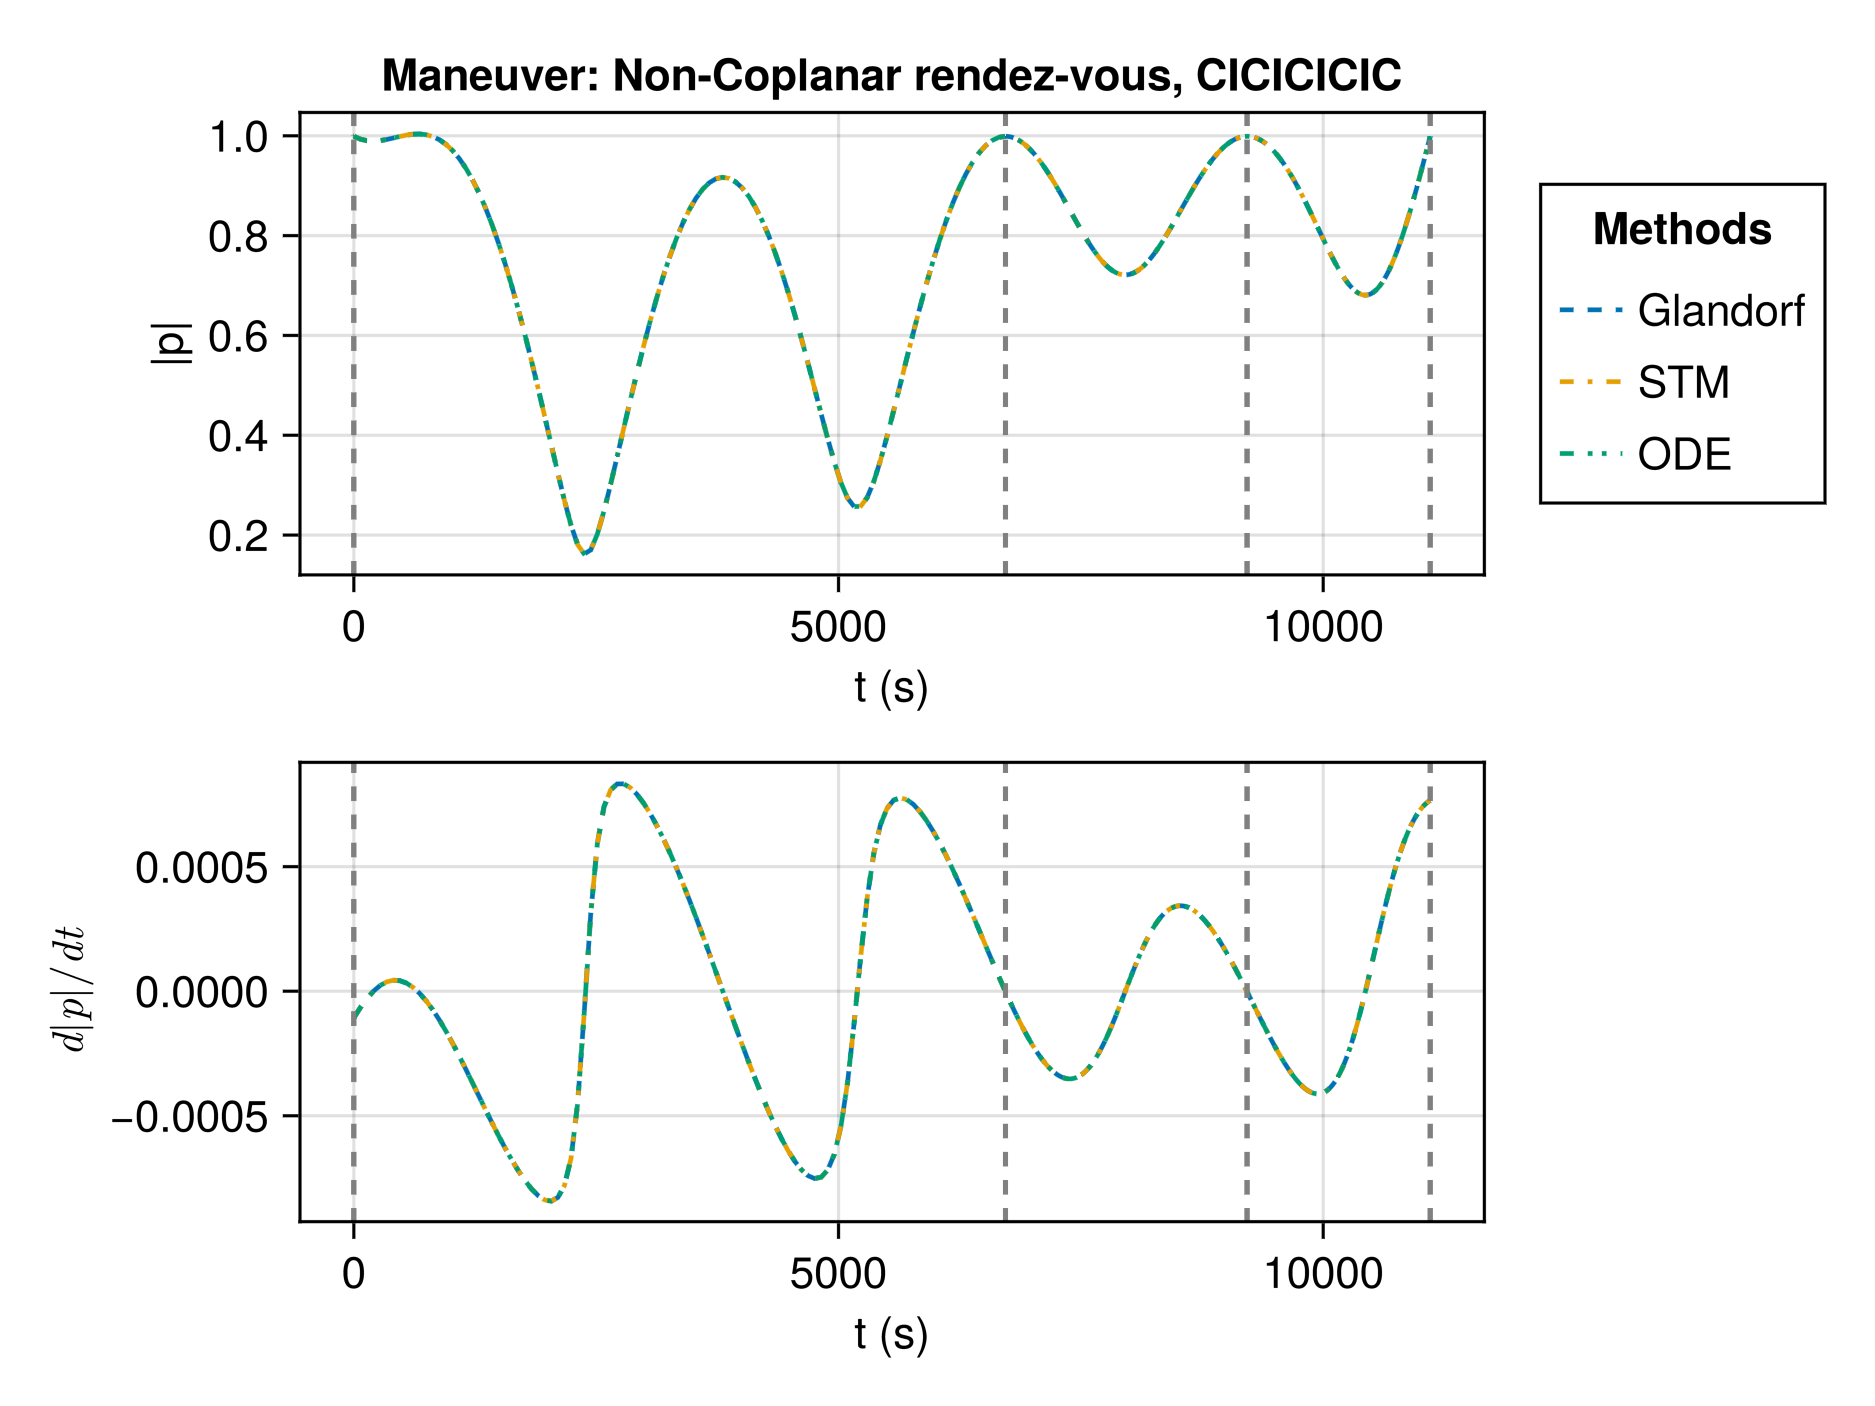
\includegraphics[width=\linewidth]{../results/two_body/ipv_noncop/CICICICIC_primer_vector.png}
    \caption{Primer vector trajectory for two body noncoplanar \texttt{CICICICIC} rendez-vous.}
    \label{fig:tb_ncop_CICICICIC_pv}
\end{figure}

\newpage
\FloatBarrier
\section{J2 Perturbed}

\subsection{Circle to Circle}

\begin{table}[htpb]
    \centering
    \begin{tabular}{cccc} \toprule
    \multicolumn{2}{c}{\textbf{Maneuver type}} & \multicolumn{2}{c}{ICI} \\ \midrule
    \(L\) (m) & \(T\) (s) & \(\varepsilon\) & \(\Delta x_{f}\) (m)    \\ \midrule
    8.0e6          & 1.0          & 1.00e-05                & 0.49713                        \\ \midrule
    \(\max \lVert p \rVert\) & 563.46     & \textbf{Diagnostic}   & Initial + Final coast        \\ \midrule
    \textbf{Impulse} & \(t\) (s) & \(\Delta v\) (m/s) & \(1 - p \cdot \hat{u}\) \\ \midrule
    1                 & 0.0          & 5209.47789             & -0.0                    \\
    2                 & 3560.54079          & 4318.71793             & -0.0                    \\\midrule
    \textbf{Total}   & 3560.54079          & 9528.19582             &                     \\ \bottomrule   
    \end{tabular}
\end{table}


\begin{table}[htpb]
    \centering
    \begin{tabular}{cccc} \toprule
    \multicolumn{2}{c}{\textbf{Maneuver type}} & \multicolumn{2}{c}{CICIC} \\ \midrule
    \(L\) (m) & \(T\) (s) & \(\varepsilon\) & \(\Delta x_{f}\) (m)    \\ \midrule
    8.0e6          & 1.0          & 1.00e-05                & 4.0e-5                        \\ \midrule
    \(\max \lVert p \rVert\) & 2.0864     & \textbf{Diagnostic}   & Add impulse        \\ \midrule
    \textbf{Impulse} & \(t\) (s) & \(\Delta v\) (m/s) & \(1 - p \cdot \hat{u}\) \\ \midrule
    1                 & 72.53153          & 473.46697             & -0.0                    \\
    2                 & 3448.63865          & 438.46605             & -0.0                    \\\midrule
    \textbf{Total}   & 3560.54079          & 911.93302             &                     \\ \bottomrule   
    \end{tabular}
\end{table}



\begin{table}[htpb]
    \centering
    \begin{tabular}{cccc} \toprule
    \multicolumn{2}{c}{\textbf{Maneuver type}} & \multicolumn{2}{c}{CICICIC} \\ \midrule
    \(L\) (m) & \(T\) (s) & \(\varepsilon\) & \(\Delta x_{f}\) (m)    \\ \midrule
    8.0e6          & 1.0          & 1.00e-05                & 0.02201                        \\ \midrule
    \(\max \lVert p \rVert\) & 1.0     & \textbf{Diagnostic}   & Local optimum        \\ \midrule
    \textbf{Impulse} & \(t\) (s) & \(\Delta v\) (m/s) & \(1 - p \cdot \hat{u}\) \\ \midrule
    1                 & 0.38763          & 451.26267             & -0.0                    \\
    2                 & 1697.05494          & 25.16996             & -0.0                    \\
    3                 & 3559.91404          & 416.62074             & -0.0                    \\\midrule
    \textbf{Total}   & 3560.54079          & 893.05336             &                     \\ \bottomrule   
    \end{tabular}
\end{table}



\subsection{Noncoplanar rendez-vous}


\begin{table}[htpb]
    \centering
    \begin{tabular}{cccc} \toprule
    \multicolumn{2}{c}{\textbf{Maneuver type}} & \multicolumn{2}{c}{ICI} \\ \midrule
    \(L\) (m) & \(T\) (s) & \(\varepsilon\) & \(\Delta x_{f}\) (m)    \\ \midrule
    6.7631e6          & 11107.158          & 1.00e-05                & 3.63678                        \\ \midrule
    \(\max \lVert p \rVert\) & 65.441     & \textbf{Diagnostic}   & Add impulse        \\ \midrule
    \textbf{Impulse} & \(t\) (s) & \(\Delta v\) (m/s) & \(1 - p \cdot \hat{u}\) \\ \midrule
    1                 & 0.0          & 743.66668             & -0.0                    \\
    2                 & 11107.1576          & 727.80415             & -0.0                    \\\midrule
    \textbf{Total}   & 11107.1576          & 1471.47082             &                     \\ \bottomrule   
    \end{tabular}
\end{table}


\begin{table}[htpb]
    \centering
    \begin{tabular}{cccc} \toprule
    \multicolumn{2}{c}{\textbf{Maneuver type}} & \multicolumn{2}{c}{CICIC} \\ \midrule
    \(L\) (m) & \(T\) (s) & \(\varepsilon\) & \(\Delta x_{f}\) (m)    \\ \midrule
    6.7631e6          & 11107.158          & 1.00e-05                & 0.0                        \\ \midrule
    \(\max \lVert p \rVert\) & 3.8353     & \textbf{Diagnostic}   & Add impulse        \\ \midrule
    \textbf{Impulse} & \(t\) (s) & \(\Delta v\) (m/s) & \(1 - p \cdot \hat{u}\) \\ \midrule
    1                 & 7080.30484          & 24.12503             & -0.0                    \\
    2                 & 10011.10872          & 34.14936             & 0.0                    \\\midrule
    \textbf{Total}   & 11107.1576          & 58.27439             &                     \\ \bottomrule   
    \end{tabular}
\end{table}


\begin{table}[htpb]
    \centering
    \begin{tabular}{cccc} \toprule
    \multicolumn{2}{c}{\textbf{Maneuver type}} & \multicolumn{2}{c}{CICICIC} \\ \midrule
    \(L\) (m) & \(T\) (s) & \(\varepsilon\) & \(\Delta x_{f}\) (m)    \\ \midrule
    6.7631e6          & 11107.158          & 1.00e-05                & 0.0                        \\ \midrule
    \(\max \lVert p \rVert\) & 1.0     & \textbf{Diagnostic}   & Final coast        \\ \midrule
    \textbf{Impulse} & \(t\) (s) & \(\Delta v\) (m/s) & \(1 - p \cdot \hat{u}\) \\ \midrule
    1                 & 1676.61473          & 5.84342             & -0.0                    \\
    2                 & 7185.69293          & 20.83452             & -0.0                    \\
    3                 & 9942.01138          & 29.32859             & -0.0                    \\\midrule
    \textbf{Total}   & 11107.1576          & 56.00653             &                     \\ \bottomrule   
    \end{tabular}
\end{table}


\newpage
\FloatBarrier
\section{J2 and Drag}

\subsection{Circle to Circle}

STM = 
\begin{equation}
    \left[
    \begin{array}{cccccc}
    0.0 & 0.0 & 0.0 & 1.0 & 0.0 & 0.0 \\
    0.0 & 0.0 & 0.0 & 0.0 & 1.0 & 0.0 \\
    0.0 & 0.0 & 0.0 & 0.0 & 0.0 & 1.0 \\
    2.330467902138264e-6 & 0.0 & 0.0 & -5.56731285604946e-12 & 0.0 & 0.0 \\
    3.461582630528354e-13 & -1.1636671818027878e-6 & 0.0 & 0.0 & -7.772214569467844e-12 & -2.7228268563396247e-12 \\
    4.2746985475505877e-13 & 0.0 & -1.1668007203354768e-6 & 0.0 & -2.722826856339625e-12 & -8.929723998680535e-12 \\
    \end{array}
    \right]
\end{equation}

PVDOT MATRIX = 
\begin{equation}
    \left[
    \begin{array}{cccccc}
    0.0 & 0.0 & 0.0 & 1.0 & 0.0 & 0.0 \\
    0.0 & 0.0 & 0.0 & 0.0 & 1.0 & 0.0 \\
    0.0 & 0.0 & 0.0 & 0.0 & 0.0 & 1.0 \\
    2.330467902138264e-6 & 3.461582630528354e-13 & 4.2746985475505877e-13 & 5.56731285604946e-12 & 0.0 & 0.0 \\
    0.0 & -1.1636671818027878e-6 & 0.0 & 0.0 & 7.772214569467844e-12 & 2.722826856339625e-12 \\
    0.0 & 0.0 & -1.1668007203354768e-6 & 0.0 & 2.7228268563396247e-12 & 8.929723998680535e-12 \\
    \end{array}
    \right]
\end{equation}

    
\begin{table}[htpb]
    \centering
    \begin{tabular}{cccc} \toprule
    \multicolumn{2}{c}{\textbf{Maneuver type}} & \multicolumn{2}{c}{ICI} \\ \midrule
    \(L\) (m) & \(T\) (s) & \(\varepsilon\) & \(\Delta x_{f}\) (m)    \\ \midrule
    8.0e6          & 1.0          & 1.00e-05                & 0.49712                        \\ \midrule
    \(\max \lVert p \rVert\) & 563.46     & \textbf{Diagnostic}   & Initial + Final coast        \\ \midrule
    \textbf{Impulse} & \(t\) (s) & \(\Delta v\) (m/s) & \(1 - p \cdot \hat{u}\) \\ \midrule
    1                 & 0.0          & 5209.4779             & -0.0                    \\
    2                 & 3560.54079          & 4318.71793             & -0.0                    \\\midrule
    \textbf{Total}   & 3560.54079          & 9528.19583             &                     \\ \bottomrule   
    \end{tabular}
\end{table}

\section{Discussion}